%%=============================================================================
%% Methodologie
%%=============================================================================

\chapter{\IfLanguageName{dutch}{Methodologie}{Methodology}}
\label{ch:methodologie}

%% TODO: Hoe ben je te werk gegaan? Verdeel je onderzoek in grote fasen, en
%% licht in elke fase toe welke stappen je gevolgd hebt. Verantwoord waarom je
%% op deze manier te werk gegaan bent. Je moet kunnen aantonen dat je de best
%% mogelijke manier toegepast hebt om een antwoord te vinden op de
%% onderzoeksvraag.


\section{\IfLanguageName{dutch}{Installatie}{Installation}}
\label{sec:M-installatie}

De eerste stap om dit onderzoek uit te voeren is het installeren van de correcte software. Hieronder wordt een overzicht van de delen binnen de installatie getoond:
\begin{itemize}
    \item Hardware
    \item Android Studio
    \item Xcode
    \item JDK
\end{itemize}
Binnen dit deel van de methodologie zullen per deel de vereiste stappen besproken worden om de software te installeren.

    \subsection{\IfLanguageName{dutch}{Hardware}{Hardware}}
    \label{sec:I-hardware}
    Vooraleer deze software te installeren is het belangrijk te weten dat een computer of laptop die draait op macOS\footnote{apple.com/benl/macos}noodzakelijk is. Hierbij is het ook aangeraden te controleren dat de geïnstalleerde versie minstens macOs Big Sur\footnote{apple.com/benl/macos/big-sur} 11.3.1 is. Dit zal later van belang zijn gezien de testen gedraaid worden op emulators met  iOS 14.3\footnote{apple.com/benl/ios/ios-14} en hiervoor macOS 11.3.1 vereist is. De software kan echter ook geïnstalleerd worden op een computer of laptop die draait op Windows\footnote{microsoft.com/nl-be/windows} maar dan kunnen geen applicaties, noch native noch cross-platform, gemaakt worden voor iOS\footnote{apple.com/benl/ios}.
    \\ \\
    Een ander gegeven is dat nog niet alle software, voornamelijk Android Studio\footnote{developer.android.com/studio}, de laatste Apple Silicon\footnote{developer.apple.com/documentation/apple-silicon} processors ondersteunen. Een eventuele omweg kan gebeuren via Apple Rosetta 2\footnote{developer.apple.com/documentation/apple-silicon/about-the-rosetta-translation-environment} maar dit lost niet alle problemen op. Indien er toch op een Apple Silicon toestel dient gewerkt te worden, is het aanbevolen de websites van de desbetreffende software te controleren voor compatibiliteit.  
    \\ \\
    Voor dit onderzoek zal bijgevolg een laptop gebruikt worden die draait op macOs. Het toestel in kwestie is een MacBook Pro 16 inch uit 2019.
    Meer technische informatie over dit toestel kan op volgende link teruggevonden worden:\\
    \verb*|https://support.apple.com/kb/SP809|
    \\ \\
    Meer informatie over de recentste versies van \textbf{macOS Big Sur} kan teruggevonden worden op volgende link:\\
    \verb*|https://support.apple.com/en-us/HT211896|

    \subsection{\IfLanguageName{dutch}{Android Studio}{Android Studio}}
    \label{sec:I-AS}
    Android Studio is het eerste deel van de vereiste software, en wordt aangeboden door JetBrains\footnote{jetbrains.com} en door Google\footnote{about.google} als software voor de ontwikkeling van Android\footnote{android.com} applicaties. Android Studio is gebaseerd op IntelliJ IDEA\footnote{jetbrains.com/idea} van JetBrains. De laatste stabiele versie van Android Studio voor macOS is 4.2.  Afhankelijk van het project dat gebruikt wordt, kunnen er echter nog enkele problemen optreden met de versie van Android Jetpack\footnote{developer.android.com/jetpack}. Dit kan opgelost worden door de Canary build van Android studio te downloaden. De laatste versie van Android Studio Canary build\footnote{developer.android.com/studio/preview} is Artic Fox (2020.3.1) Canary 15.
    \\ \\
    De laatste versie van \textbf{Android Studio} kan hier teruggevonden worden:\\
    \verb*|https://developer.android.com/studio|
    \\ \\ 
    De laatste versie van \textbf{Android Studio Canary build} kan hier teruggevonden worden:\\
    \verb*|https://developer.android.com/studio/preview|
    \\ \\
    Oudere versies van Android Studio ondersteunen de recentste plug-ins voor Kotlin Multiplatform Mobile (KMM) niet. Hierbij is het dus belangrijk dat de versie die geïnstalleerd wordt 4.2 of recenter is.
    \\ \\ 
    Tijdens de installatie van Android Studio kan er best geopteerd worden om de standaard instellingen te gebruiken. Daarnaast zullen verschillende zaken geïnstalleerd worden namelijk:
    \begin{itemize}
        \item Android Emulator
        \item Android SDK Build Tools 30.0.3
        \item Android SDK Platform 30
        \item Android SDK Platform-Tools
        \item Android SDK Tools
        \item Google APIs Intel x86 Atom System Image
        \item Intel x86 Emulator Accelerator (HAXM installer)
        \item SDK Patch Applier v4
        \item Sources for Android 30
    \end{itemize}
    Deze zijn allemaal van belang voor zowel de native Android ontwikkeling als de KMM cross-platform ontwikkeling. Eens de installatie voltooid is kan via de AVD manager een emulator geïnstalleerd worden. Voor deze studie zal er een Pixel 4a\footnote{store.google.com/us/product/pixel\_4a?hl=en-US} geïnstalleerd worden met Android 11\footnote{android.com/android-11} (API Level 30). Deze emulator zal gebruikt worden om de native Android en de KMM cross-platform applicatie te testen. Eens deze emulator correct is geïnstalleerd kan deze teruggevonden worden in de ADV Manager zoals op figuur \ref{fig:M-as-adv-manager}
    \begin{figure}
        \centering
        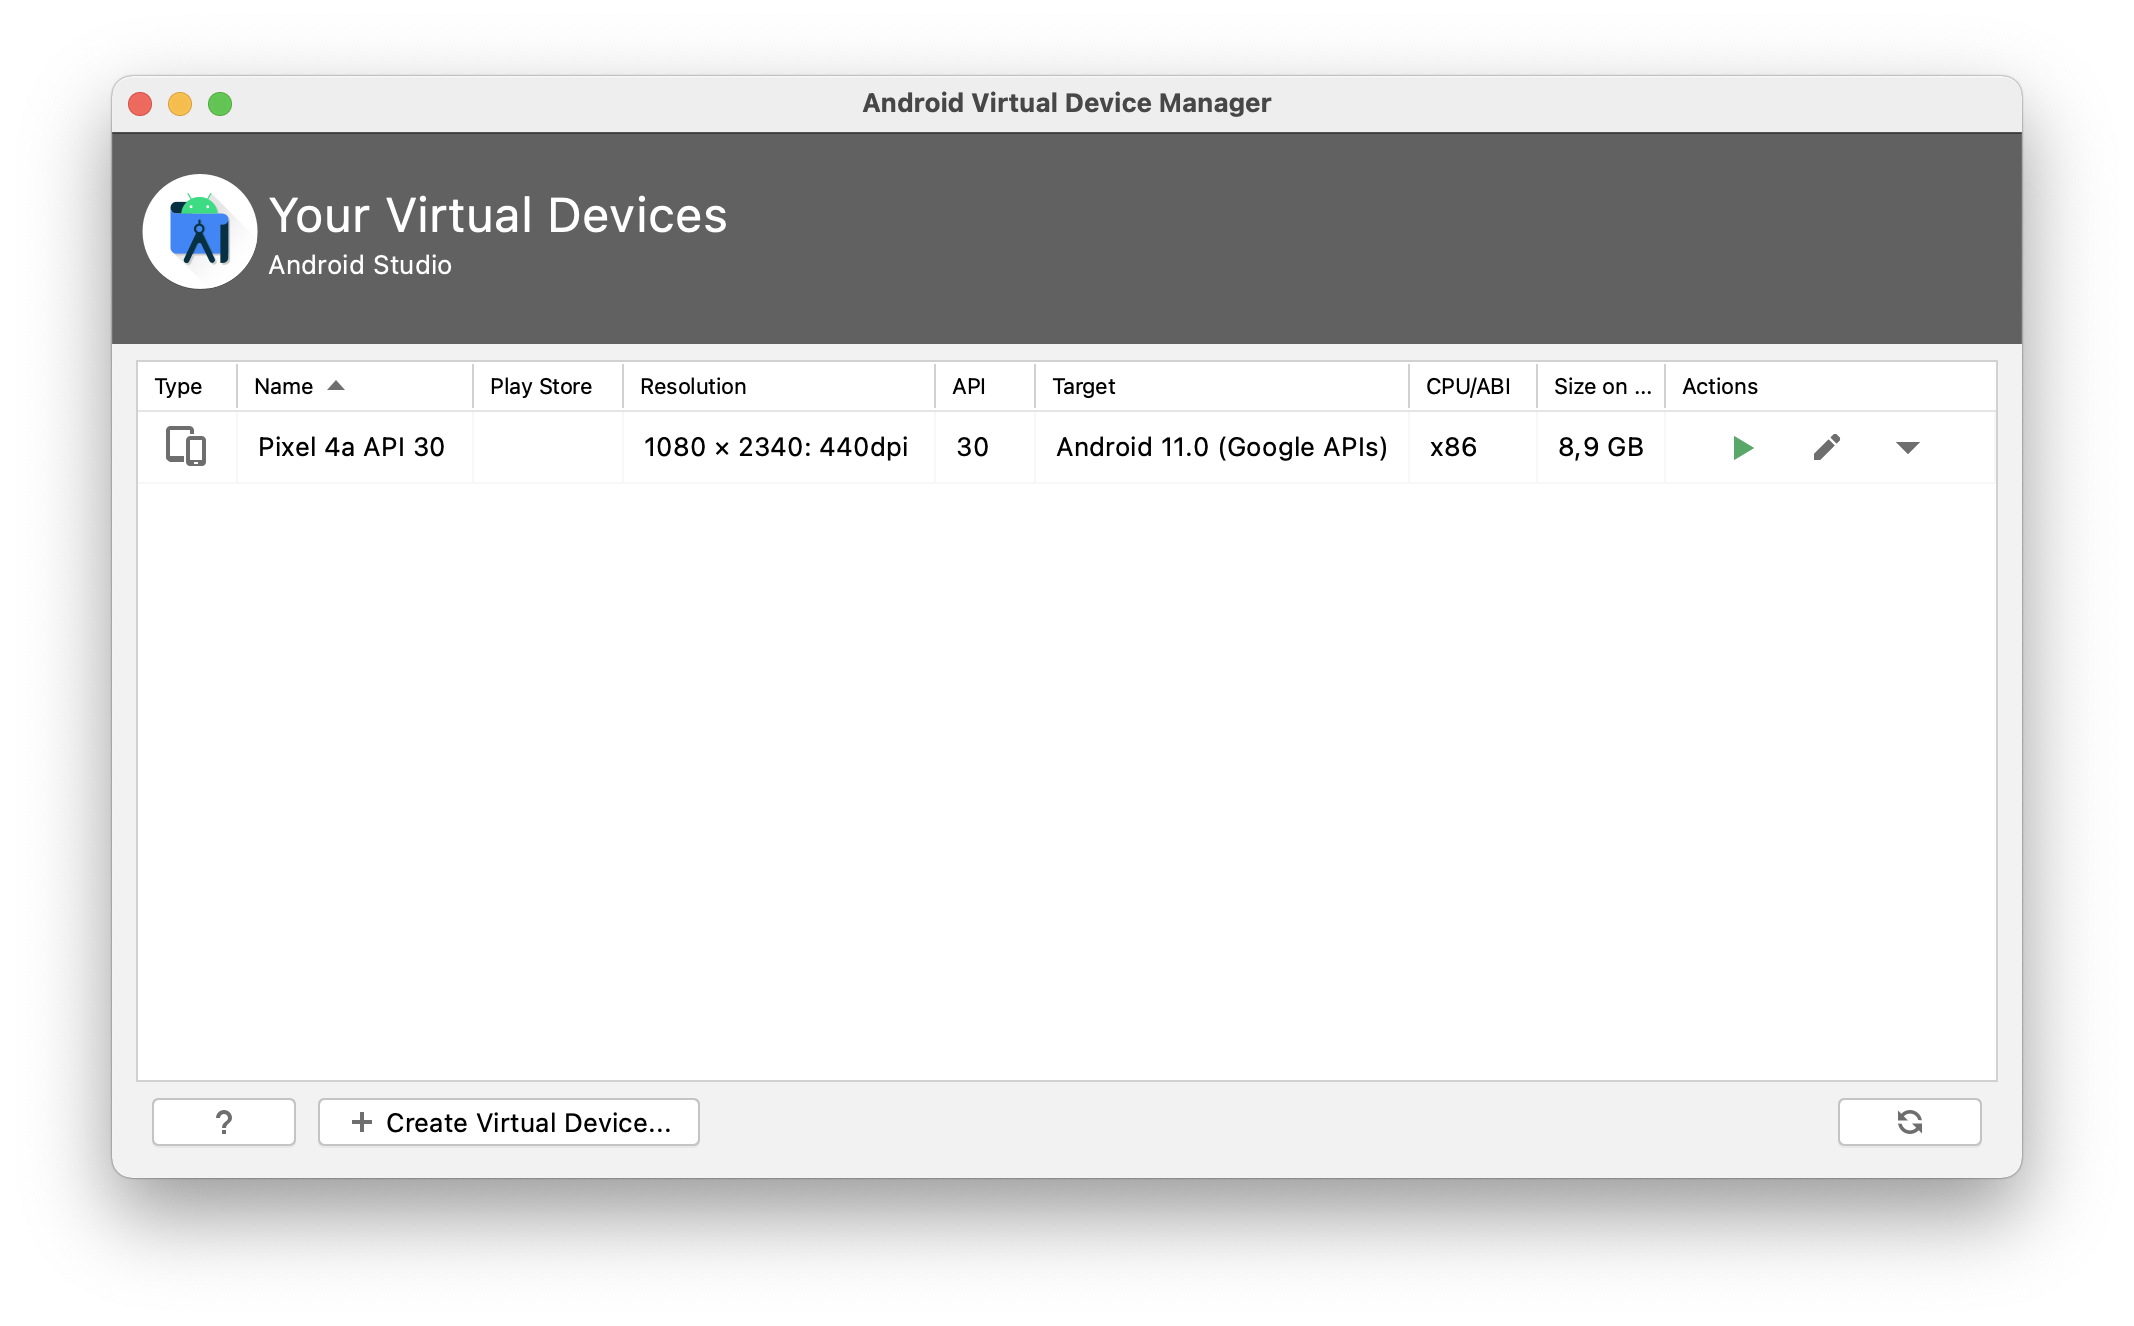
\includegraphics[width=10cm]{img/as-adv-manager.png}
        \caption{De ADV Manager in Android Studio met de Pixel 4a emulator geïnstalleerd}
        \label{fig:M-as-adv-manager}
    \end{figure}
    \\ \\
    Zoals net vermeld, is het ook nodig om de KMM plug-in te installeren voor Android Studio. De plug-in maakt het mogelijk om KMM projecten aan te maken. Hierdoor kan de business logica geschreven worden voor beide platformen, gedeeld of per platform. Een andere feature van de plug-in is dat de iOS applicatie kan gestart en gedebugd worden vanuit Android Studio. Daarnaast zullen de gebruikers door de plug-in ook de mogelijkheid krijgen om nieuwe KMM applicaties aan te maken.
    \\ \\ 
    De laatste versie van de \textbf{KMM plug-in} kan hier teruggevonden worden:\\
    \verb*|https://plugins.jetbrains.com/plugin/14936-kotlin-multiplatform-mobile|
    
    Onderstaande figuren tonen het proces om een nieuwe KMM applicatie te maken aan de hand van de KMM plug-in. 
    \begin{itemize}
        \item Figuur \ref{fig:M-kmm-plugin-1} toont de mogelijke opties binnen Android Studio voor het aanmaken van een nieuw project, eens de plugin correct is geïnstalleerd, zal daar ook de optie  `KMM Application’ beschikbaar zijn.
        \item Figuur \ref{fig:M-kmm-plugin-2} toont de standaard instellingen voor een KMM project, deze instellingen lopen gelijk met de standaard instellingen voor een standaard Android project.
        \item Figuur \ref{fig:M-kmm-plugin-3} toont de mogelijkheden om de verschillende delen van de KMM te benoemen, standaard zullen hier de waarden androidApp, iosApp en shared staan. Daarnaast kunnen deze delen nog een beschrijving krijgen. Als laatste is er de optie om templates voor testen toe te voegen aan de shared module.
    \end{itemize}
 
    \begin{figure}
        \centering
        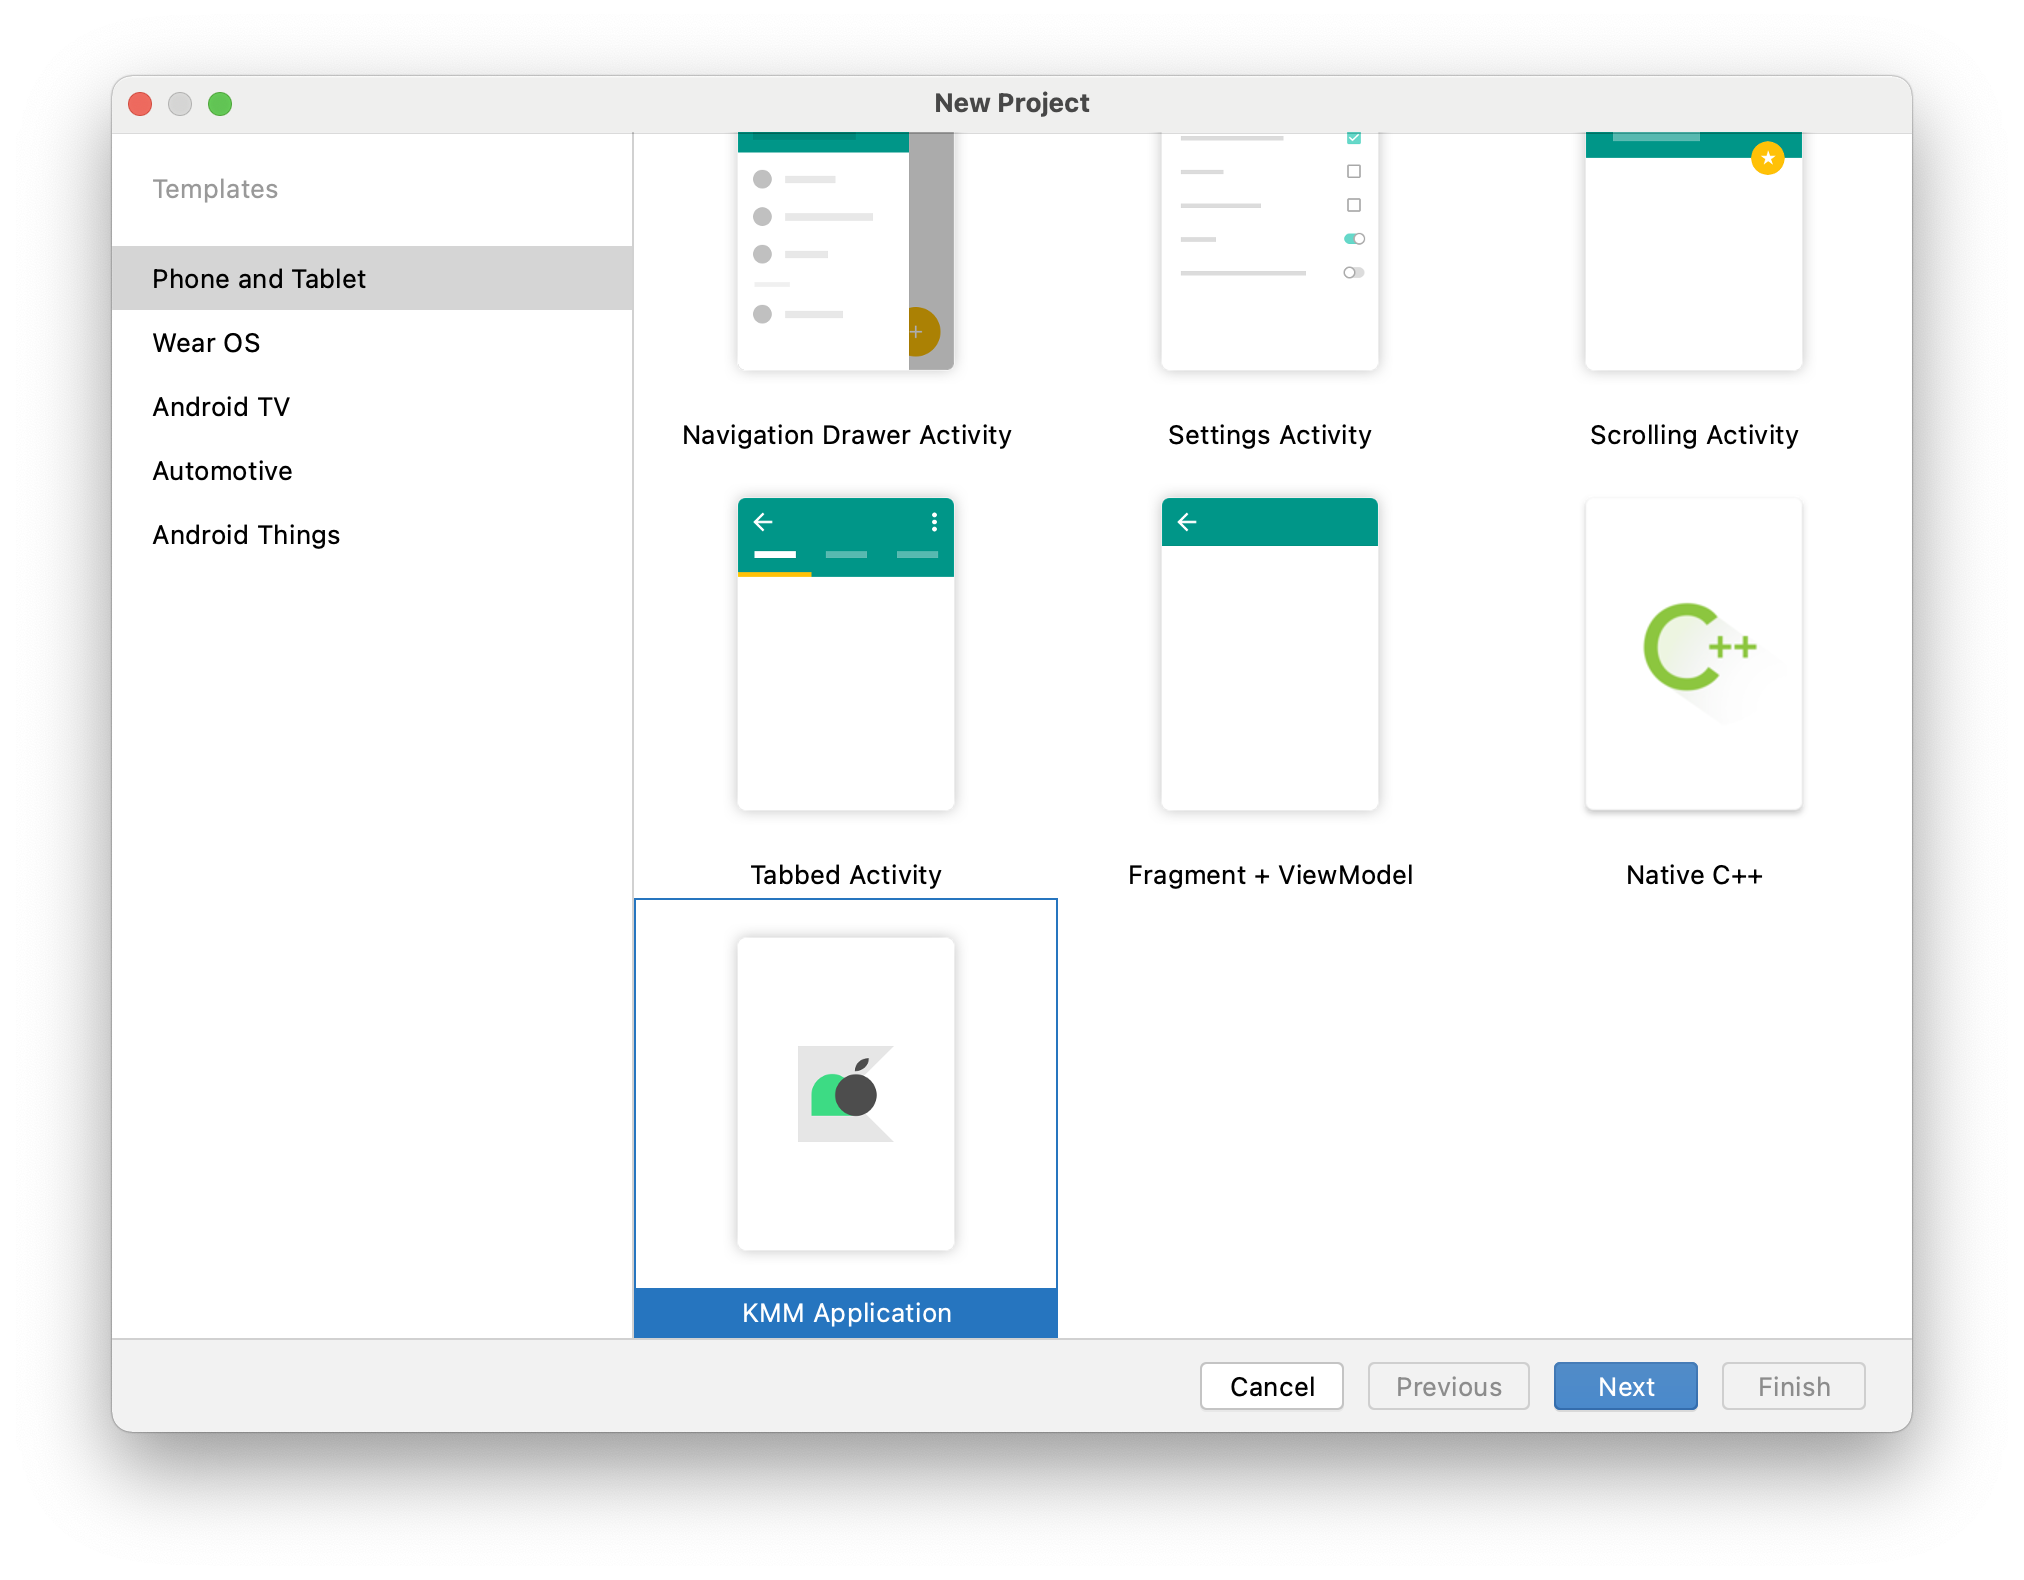
\includegraphics[width=10cm]{img/kmm-plugin-1.png}
        \caption{De opties voor een nieuw project binnen Android Studio, hierbij is een KMM applicatie ook beschikbaar}
        \label{fig:M-kmm-plugin-1}
    \end{figure}
    \begin{figure}
        \centering
        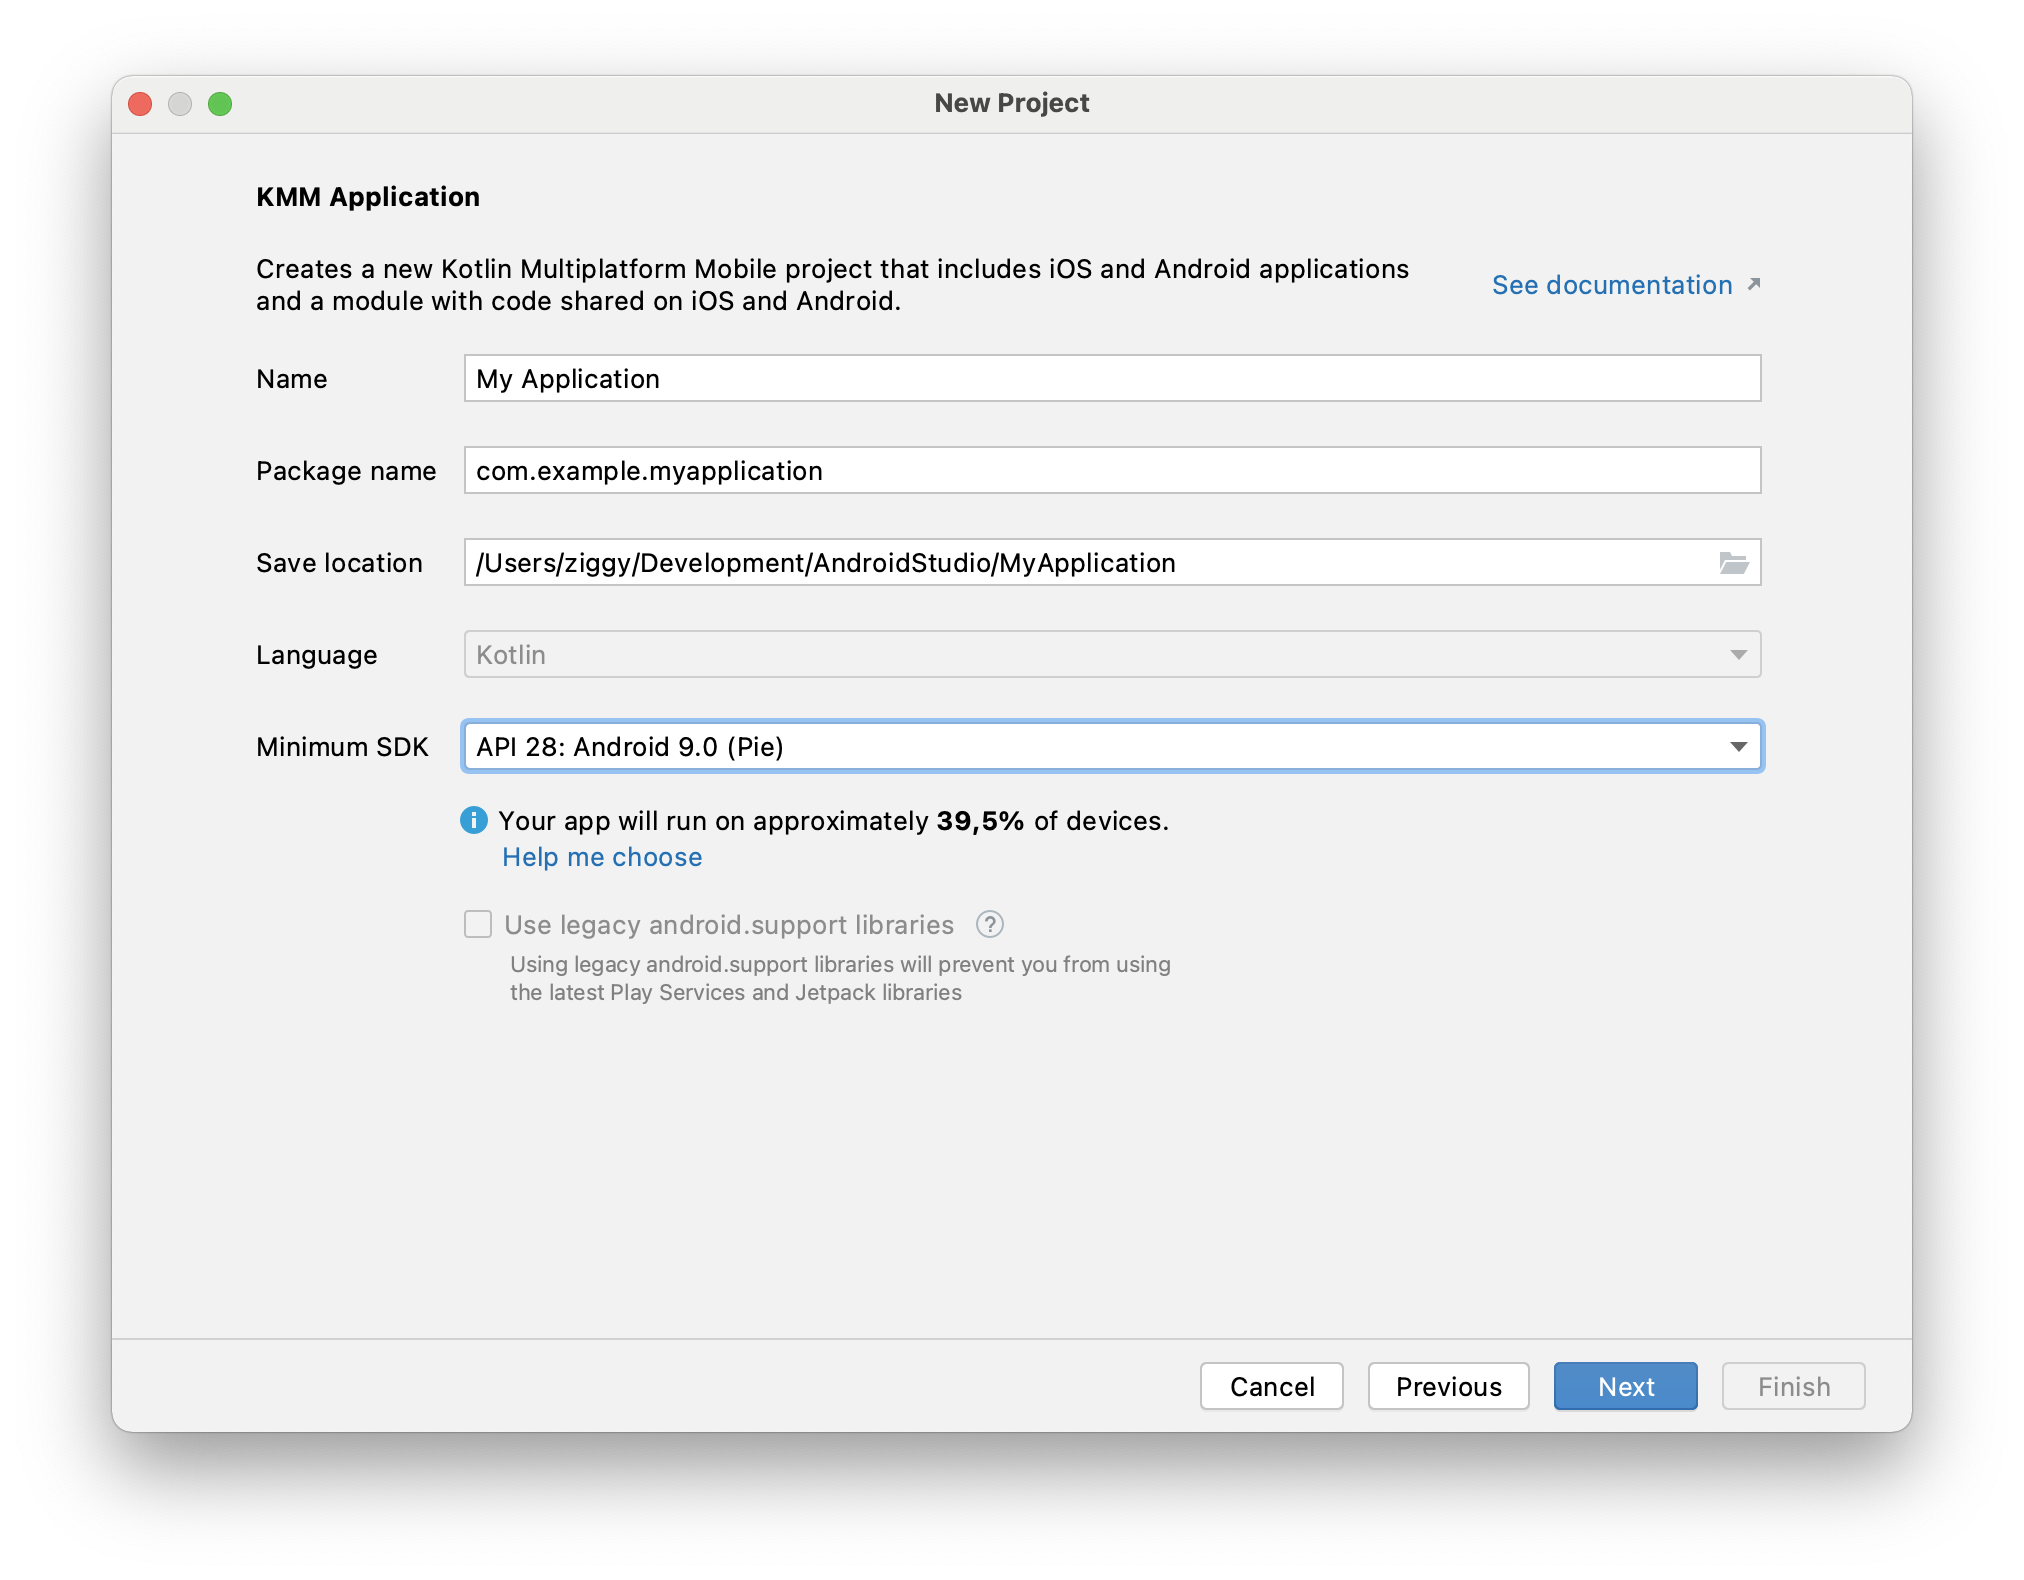
\includegraphics[width=10cm]{img/kmm-plugin-2.png}
        \caption{De standaard instellingen voor een KMM project}
        \label{fig:M-kmm-plugin-2}
    \end{figure}
    \begin{figure}
        \centering
        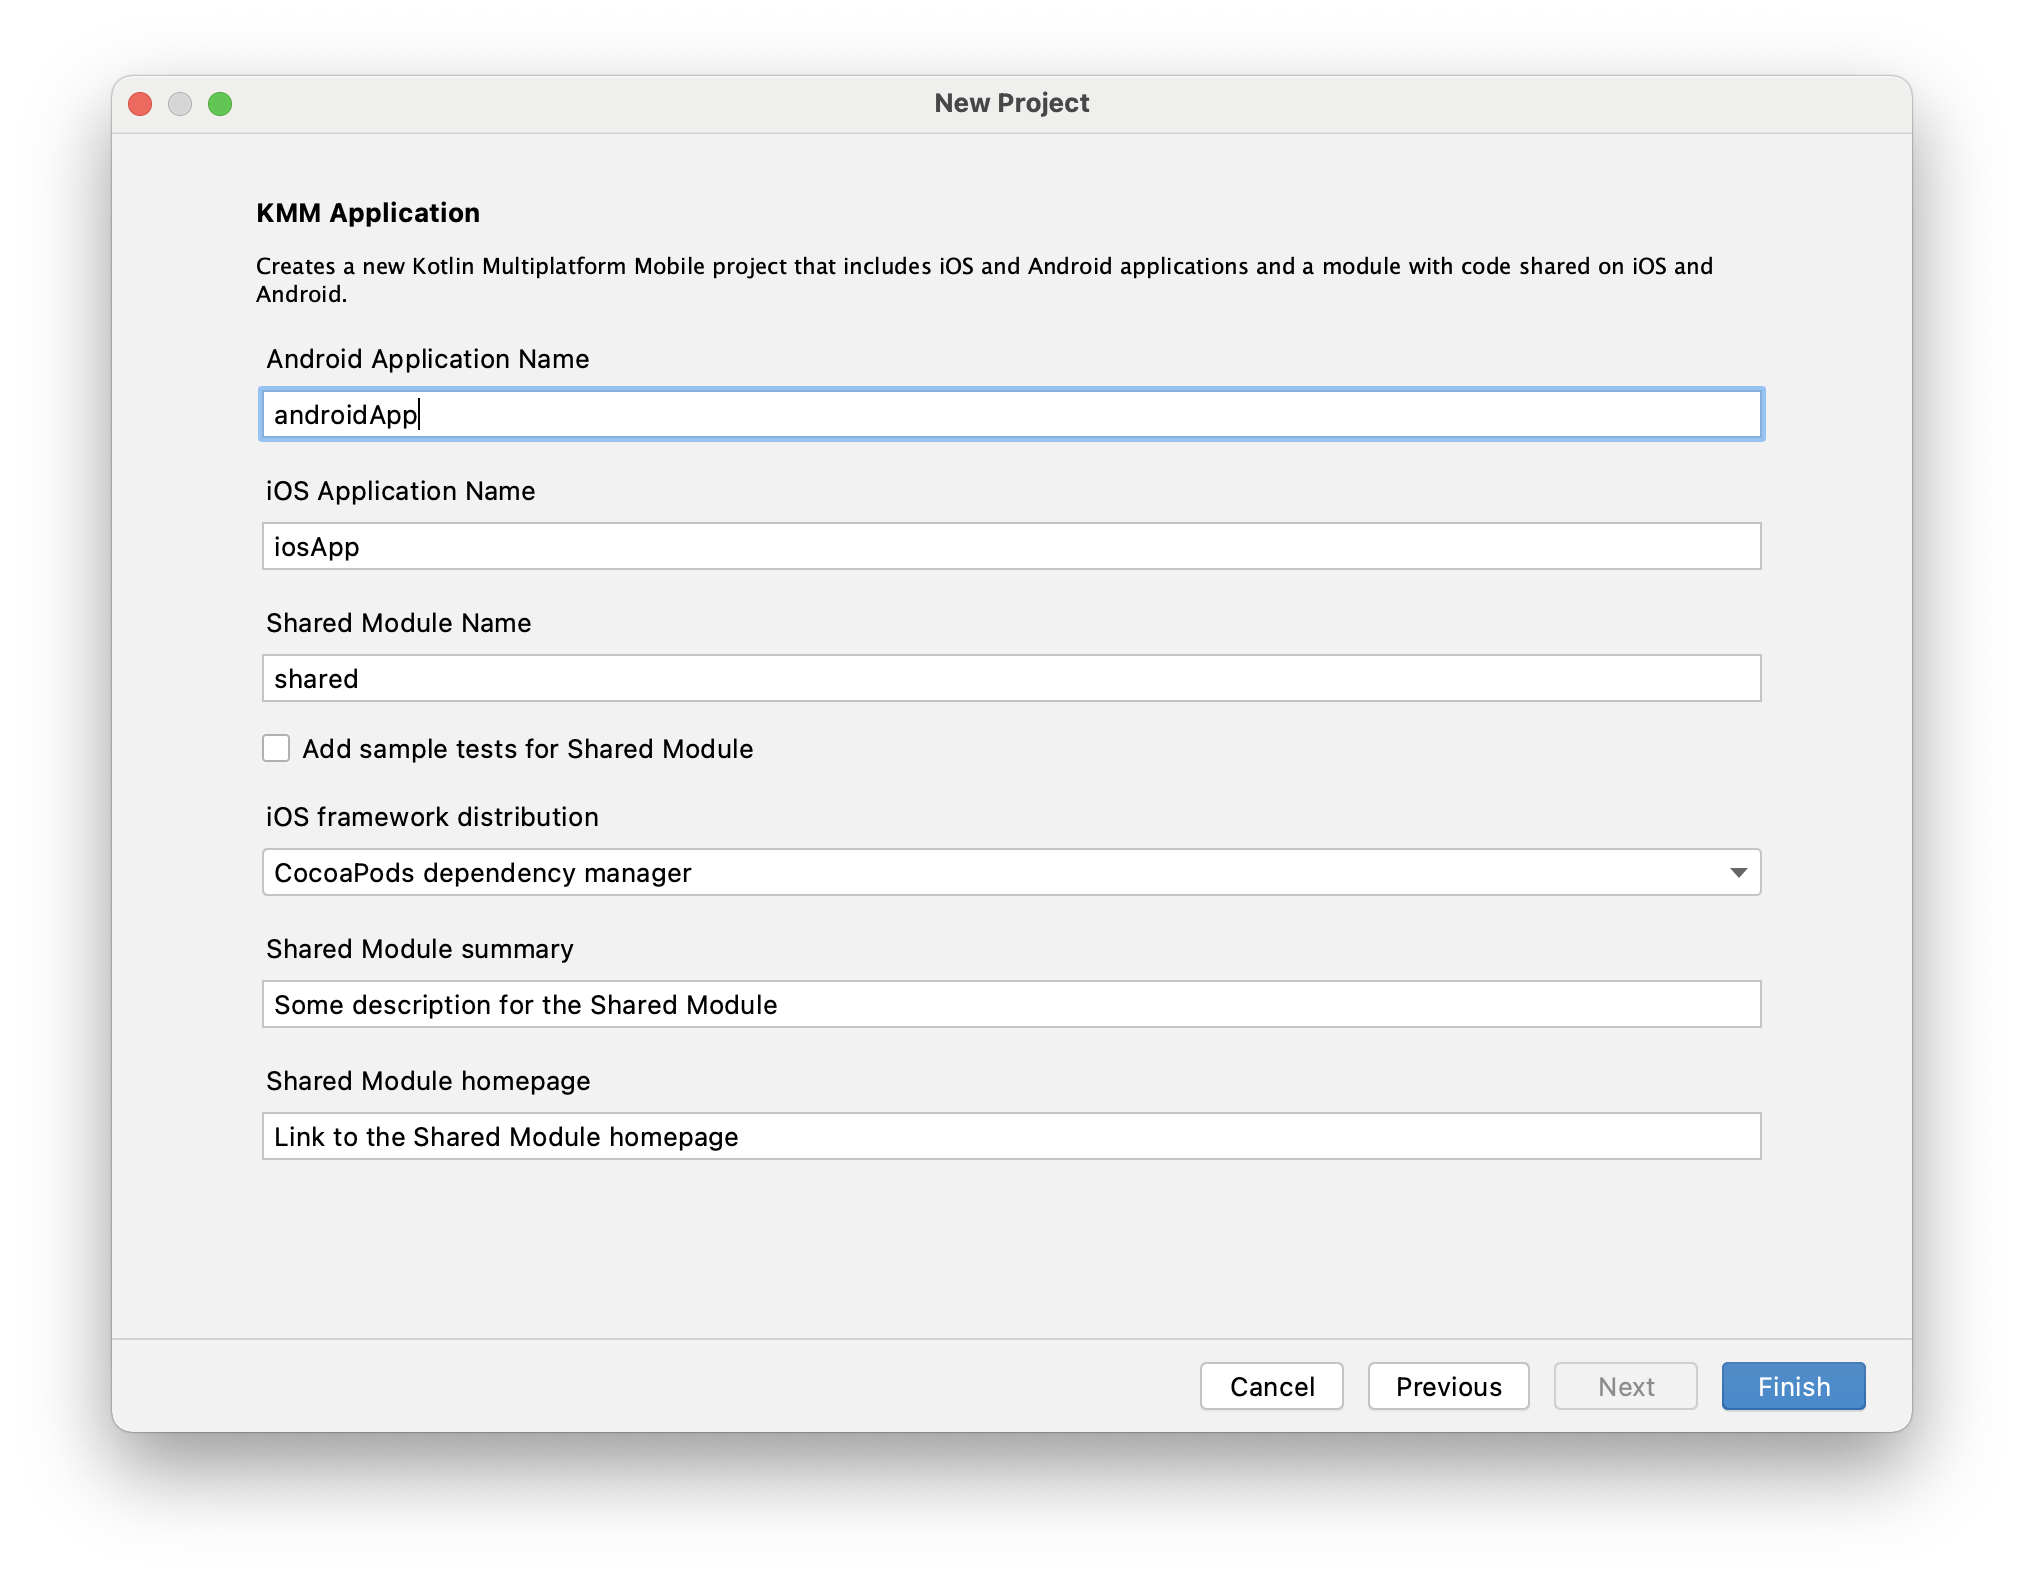
\includegraphics[width=10cm]{img/kmm-plugin-3.png}
        \caption{De instellingen van een KMM project voor de gedeelde logica en de native iOS en Android delen}
        \label{fig:M-kmm-plugin-3}
    \end{figure}

    Indien er problemen zouden zijn met de KMM plug-in kan er via de instellingen van Android Studio gecontroleerd worden of de plug-in goed geïnstalleerd is en actief staat.
    \\ \\
    \underline{Android Studio -> Voorkeuren -> Plugins -> Kotlin Multiplatform Mobile}
    \\ \\
    De plug-in zou bij de geïnstalleerde plug-ins moeten staan en moet actief staan.
    \begin{figure}
        \centering
        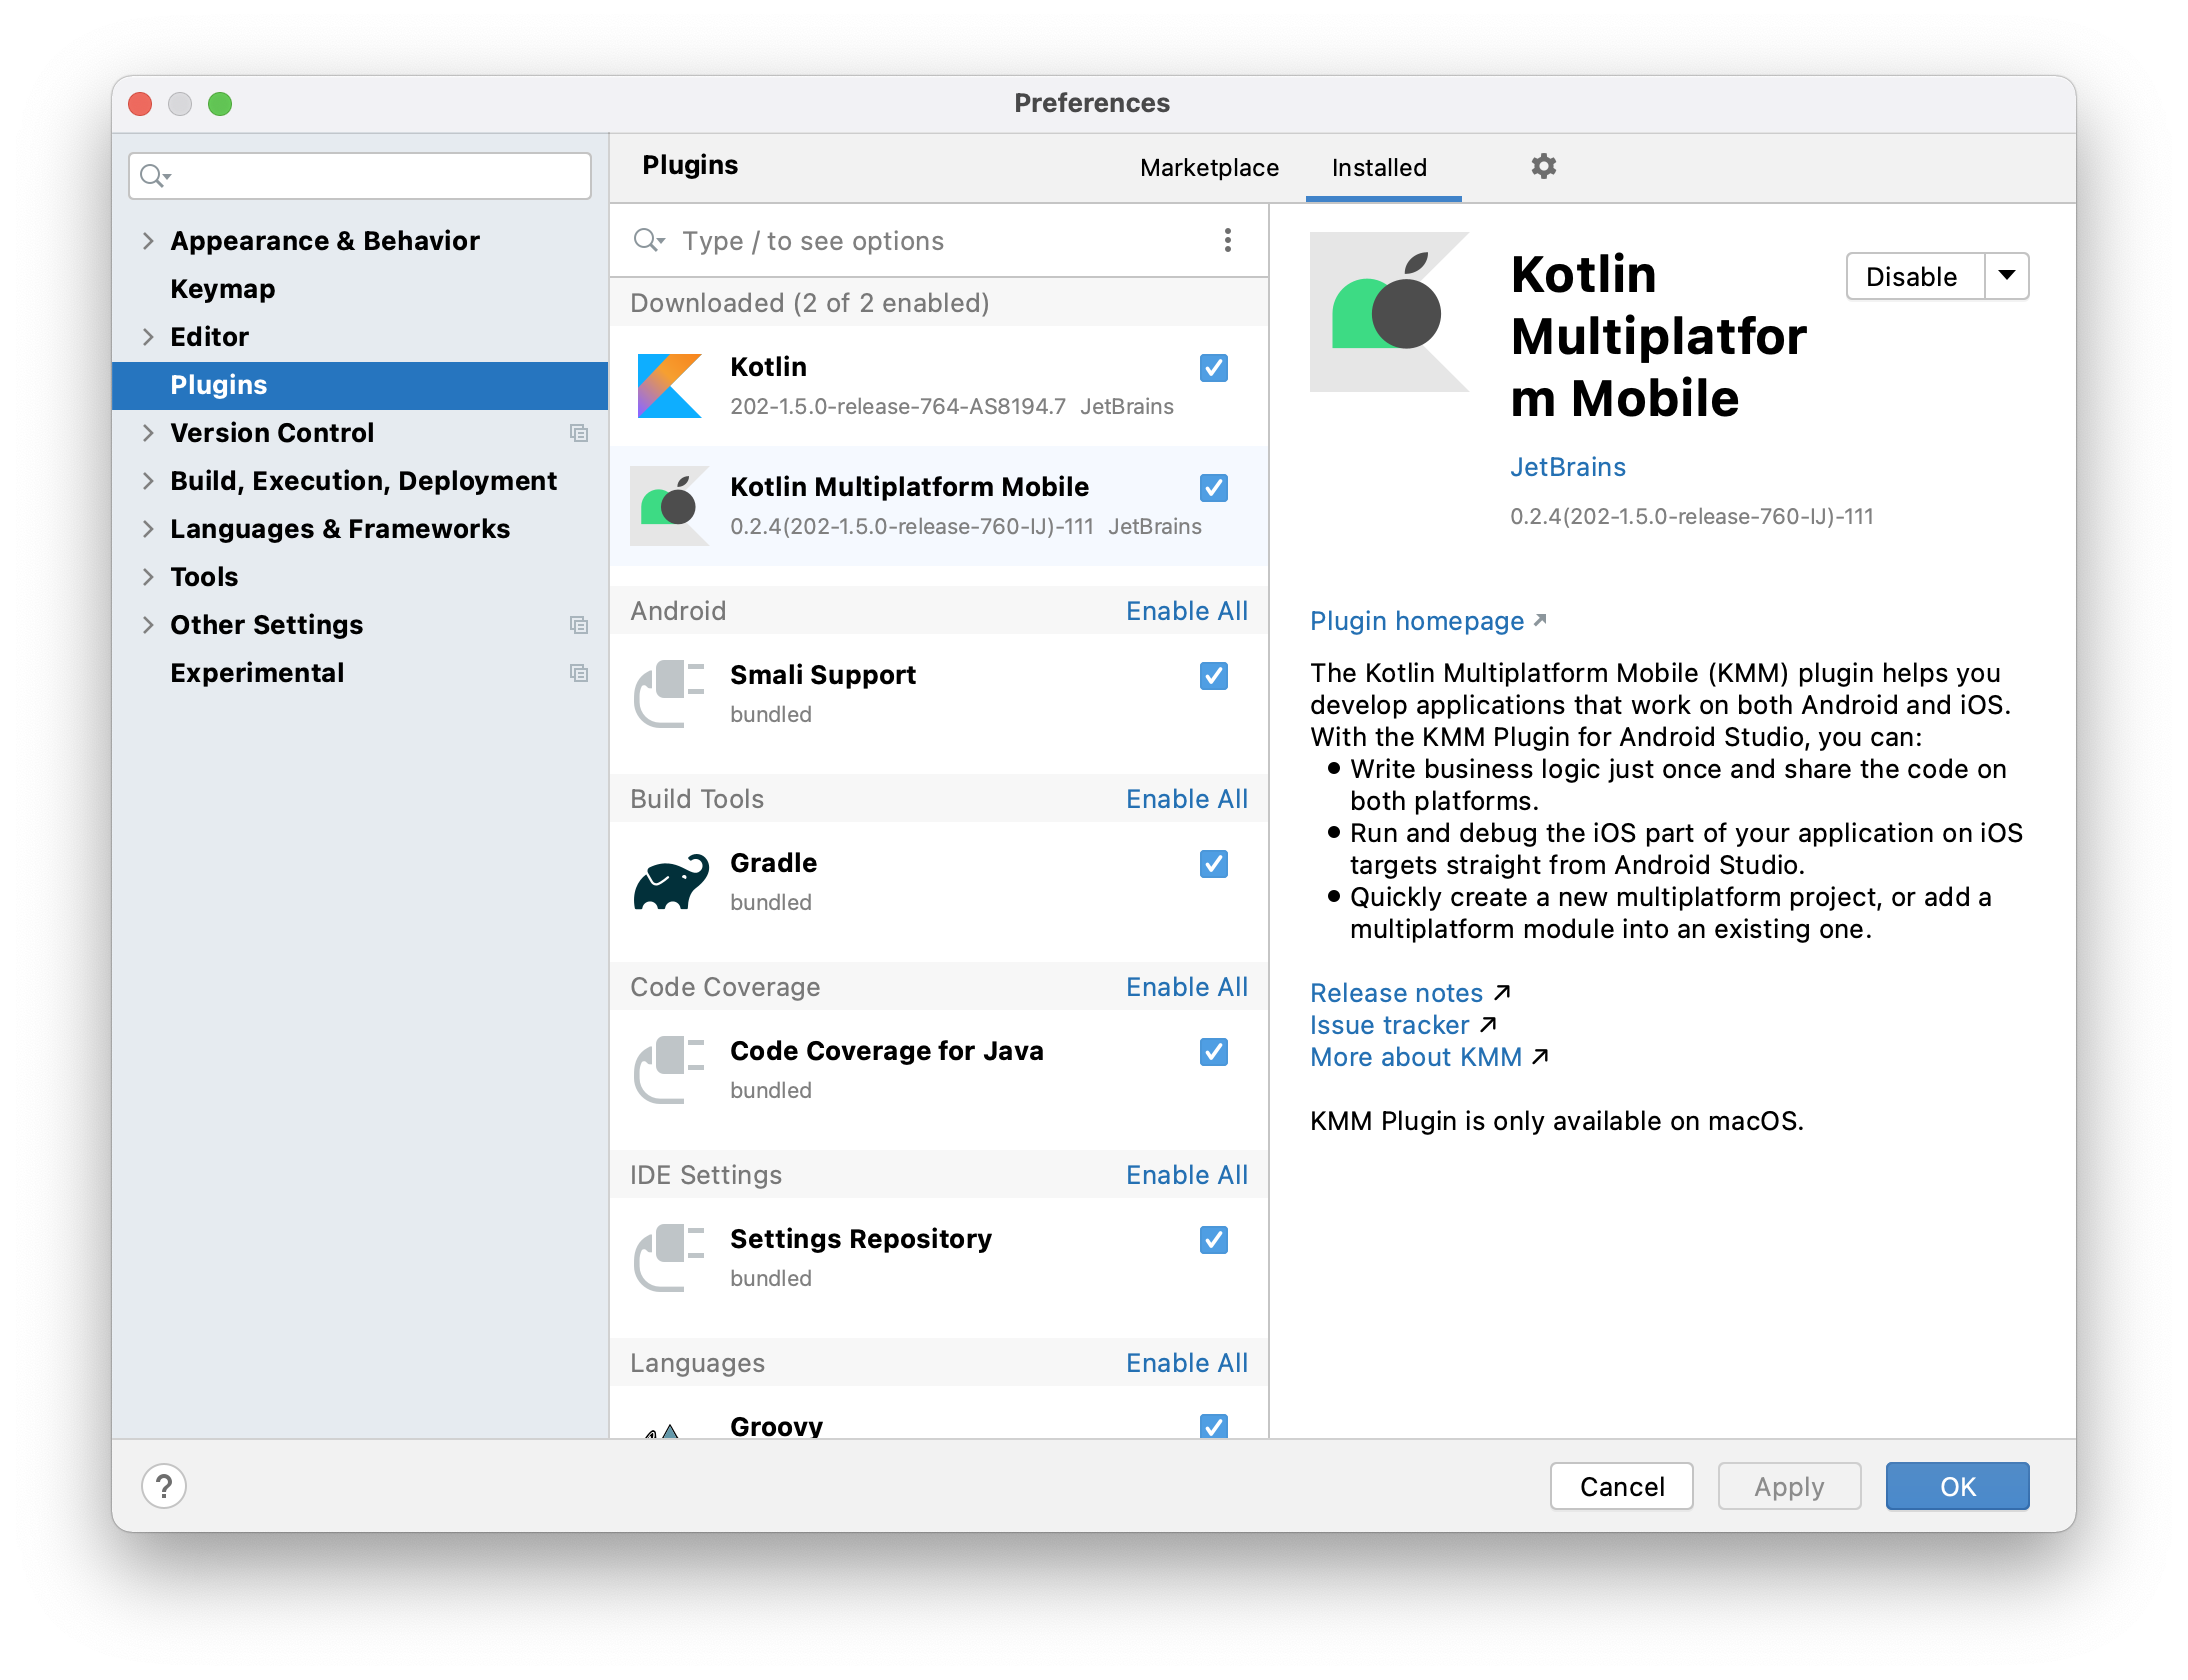
\includegraphics[width=10cm]{img/kmm-plugin-4.png}
        \caption{De plug-in geïnstalleerd binnen Android Studio}
        \label{fig:M-kmm-plugin-4}
    \end{figure}
   
   
    \subsection{\IfLanguageName{dutch}{Xcode}{Xcode}}
    \label{sec:I-Xcode}
    Het tweede deel van software dat dient geïnstalleerd te worden is Xcode\footnote{developer.apple.com/xcode}, de softwareontwikkeling omgeving van Apple\footnote{apple.com} voor toestellen die draaien op iOS, iPadOS\footnote{apple.com/benl/ipados}, macOS...  Deze software is uitsluitend beschikbaar voor toestellen die draaien op macOS. De laatste beschikbare versie is Xcode 12.5, deze ondersteunt het bouwen applicaties tot iOS 14.3, iPadOS 14.3\footnote{apple.com/benl/ipados/ios-14}, watchOS 7.4\footnote{apple.com/benl/watchos/watchos-7}... 
    \\ \\ 
    De laatste versie van \textbf{Xcode} kan geïnstalleerd worden via de Apple Developer website of via de App Store\footnote{apple.com/benl/app-store} op macOS: \\
    \verb*|https://developer.apple.com/xcode/|
    \\
    \verb*|https://apps.apple.com/nl/app/xcode/id497799835?mt=12|
    \\ \\ 
    Naast Xcode zal voor deze studie ook gebruik gemaakt worden van Xcode Command Line Tools, deze komen normaal standaard mee met de Xcode IDE. Indien de Xcode Command Line Tools niet geïnstalleerd zouden zijn kan dit via volgend terminal commando gedaan worden. \\
    \begin{lstlisting}
        //Terminal.app
        xcode-select --install
    \end{lstlisting}
    Eens deze installatie voltooid is, dient er nog binnen Xcode een aanpassing gemaakt te worden zodat de Command Line Tools actief zijn. Via \\
    \underline{Xcode -> Voorkeuren -> Locaties}, \\
    moeten de Command Line Tools ingesteld worden op `Xcode 12.5 (12E262)' deze optie zou beschikbaar moeten zijn in de selectielijst. Figuur \ref{fig:M-xcode-locations} toont het instellingenmenu voor Locaties met de correcte waarden. 
    \begin{figure}
        \centering
        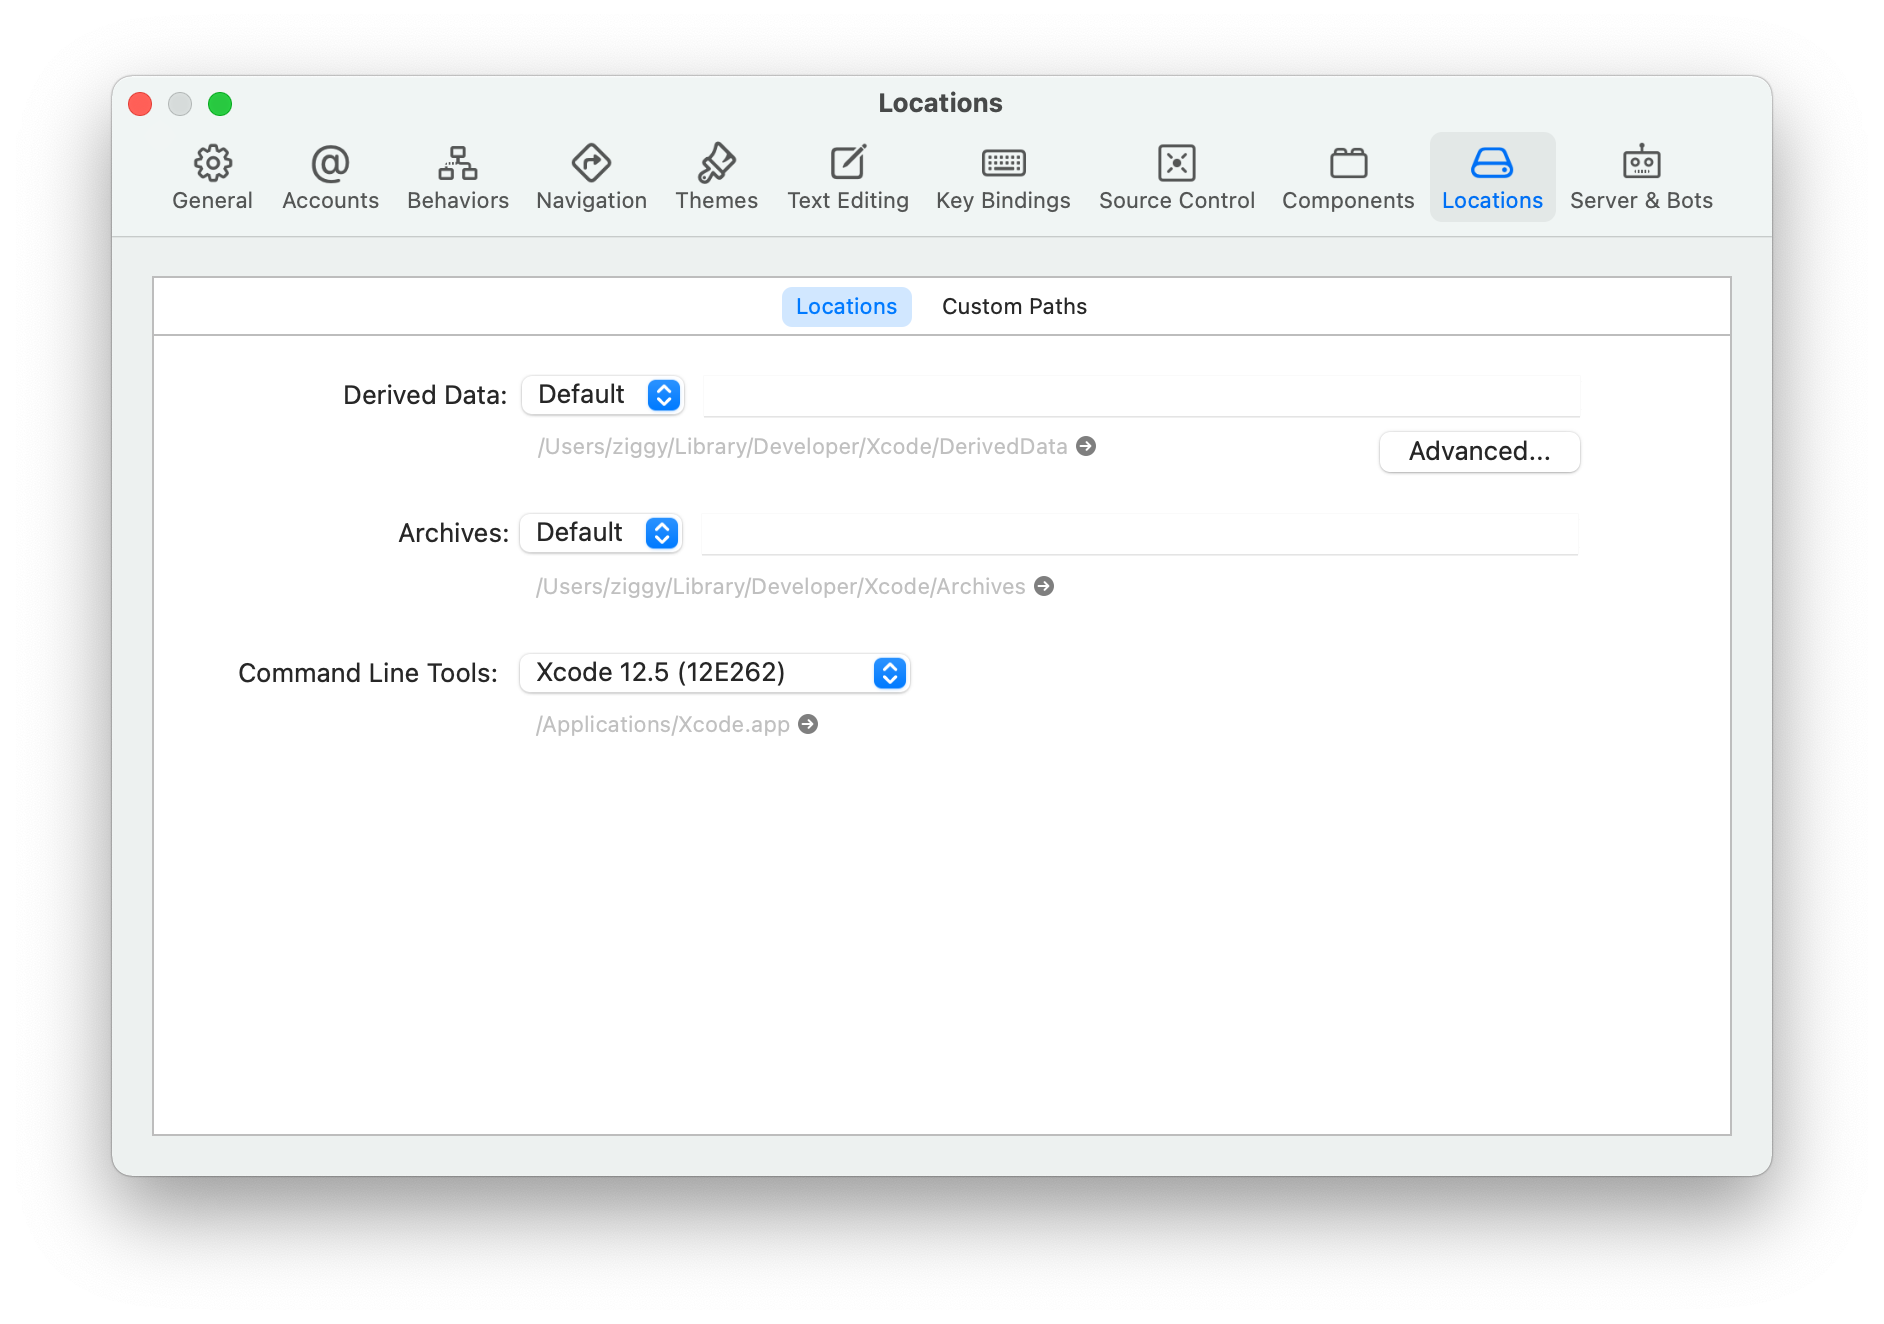
\includegraphics[width=10cm]{img/xcode-locations}
        \caption{De Xcode Command Line Tools correct geconfigureerd binnen Xcode}
        \label{fig:M-xcode-locations}
    \end{figure}
    
    Tijdens de installatie van Xcode worden alle emulators al voorzien waardoor er hier geen extra instellingen moeten aan gebeuren. Voor deze studie zal gebruik gemaakt worden van een iPhone 12\footnote{apple.com/benl/iphone-12} emulator met iOS 14.3.
    \\ \\
    Naast de installatie van Xcode zal ook CocoaPods geïnstalleerd moeten worden om de KMM plugin correct te laten werken. CocoaPods kan geinstalleerd worden aan de hand van onderstaand commando.
    
    \begin{lstlisting}
        //Terminal.app
        sudo gem install cocoapods
    \end{lstlisting}
    
    \subsection{\IfLanguageName{dutch}{JDK}{JDK}}
    \label{sec:I-JDK}
    De laatste stap van het installatieproces is het installeren van een JDK of Java Development Kit. Voor deze studie zal Java SE 16\footnote{oracle.com/java/technologies/javase-downloads.html} geïnstalleerd worden. Dit is de laatst beschikbare versie van Java\footnote{java.com}. Alle andere versies van Java SE zijn hier terug te vinden \verb*|https://www.oracle.com/java/technologies/oracle-java-archive-downloads.html|
    
    De laatste versie van de \textbf{Java JDK} kan geïnstalleerd worden via volgende website: \\
    \verb*|https://www.oracle.com/java/technologies/javase-jdk16-downloads.html|
    \\
    
    Eens de installatie voltooid is, kan de gebruiker controleren of de installatie geslaagd is door onderstaand commando uit te voeren.
    \begin{lstlisting}
        //Terminal.app
        java --version
    \end{lstlisting}
    Indien de installatie geslaagd is en Java SE 16 correct is geïnstalleerd, zal de gebruiker volgende output krijgen zoals in figuur \ref{fig:M-jdk-version} 
    
    \begin{figure}
        \centering
        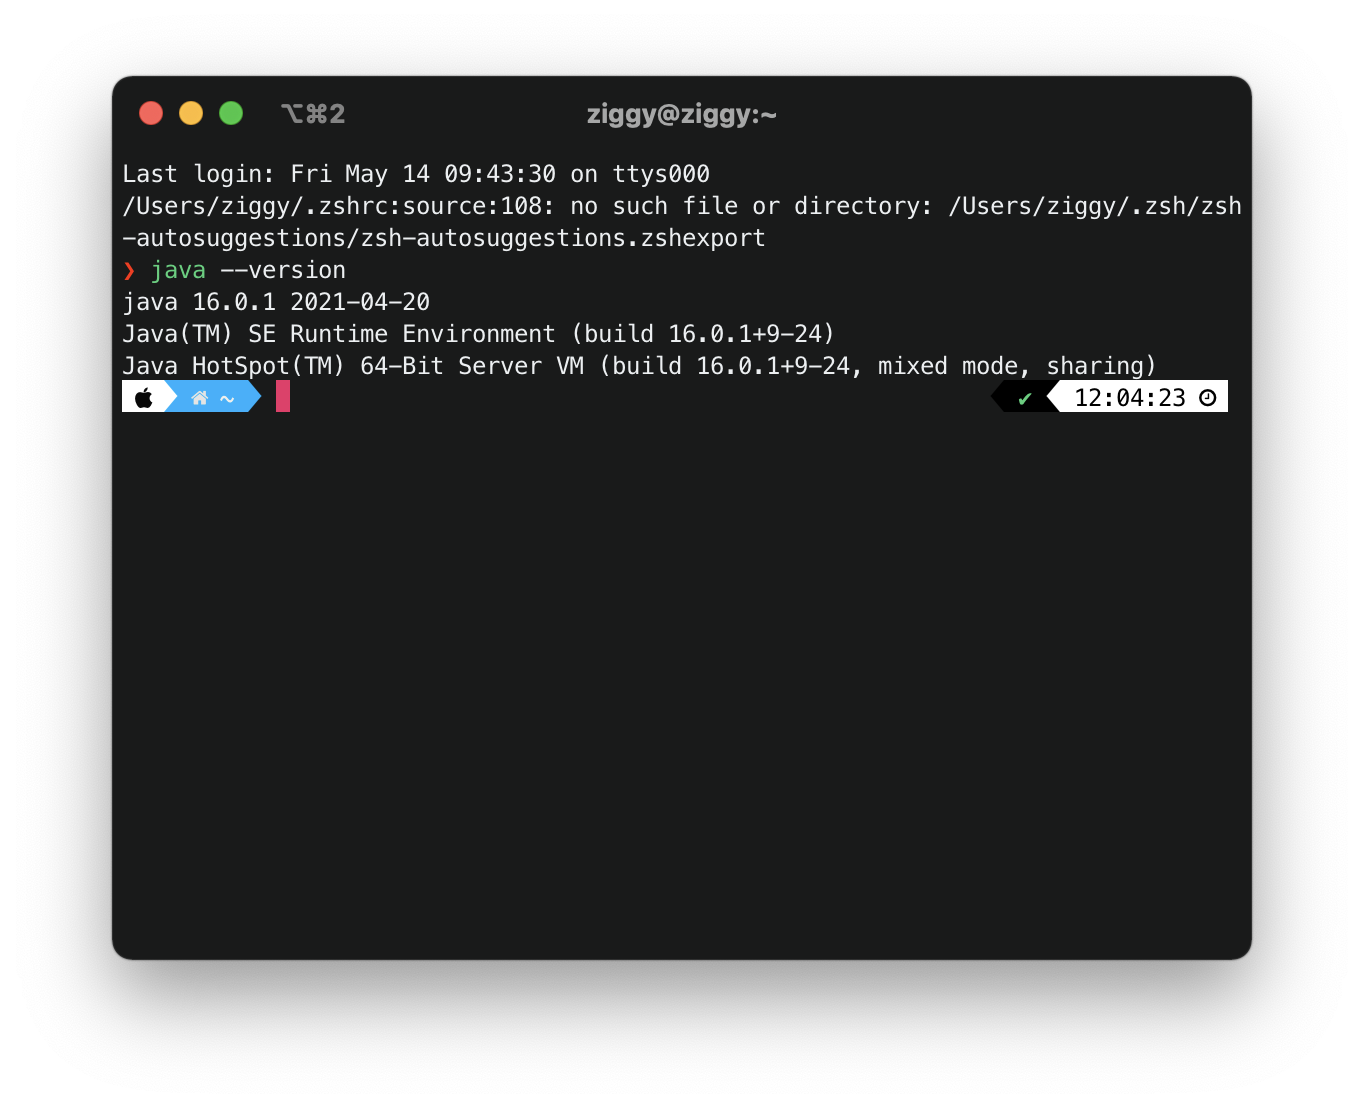
\includegraphics[width=10cm]{img/jdk-version.png}
        \caption{De terminal bevestigd dat Java SE 16 correct is geïnstalleerd op de betreffende computer}
        \label{fig:M-jdk-version}
    \end{figure}

\section{\IfLanguageName{dutch}{Basis Kotlin Multiplatform Mobile applicatie}{Basic Kotlin MultiPlatforn Mobile application}}
\label{sec:M-first-app}
Nadat alle software is geïnstalleerd kan er overgegaan worden naar de eerste Kotlin Multiplatform Mobile applicatie (KMM). De eerste applicatie zal een kleine applicatie zijn die aan de gebruiker toont welke software versie op het toestel geïnstalleerd staat.
\\ \\
De geschreven applicatie kan ook op GitHub\footnote{github.com} teruggevonden worden. Dit kan via volgende link:\\
\verb*|https://github.com/ziggymoens/KMM_Application_Basic|
\\ \\
Bij het opstarten van Android Studio geeft deze de optie om een nieuw project te starten, eens dat is aangeklikt wordt er gekozen voor de optie `KMM Application'. Als naam wordt `Basic KMM Application' gekozen en hierbij wordt de minimum SDK op level 28 (Android 9.0\footnote{android.com/versions/pie-9-0}) gezet.

\begin{figure}
    \centering
    \subfloat[\centering Startscherm Android Studio]{{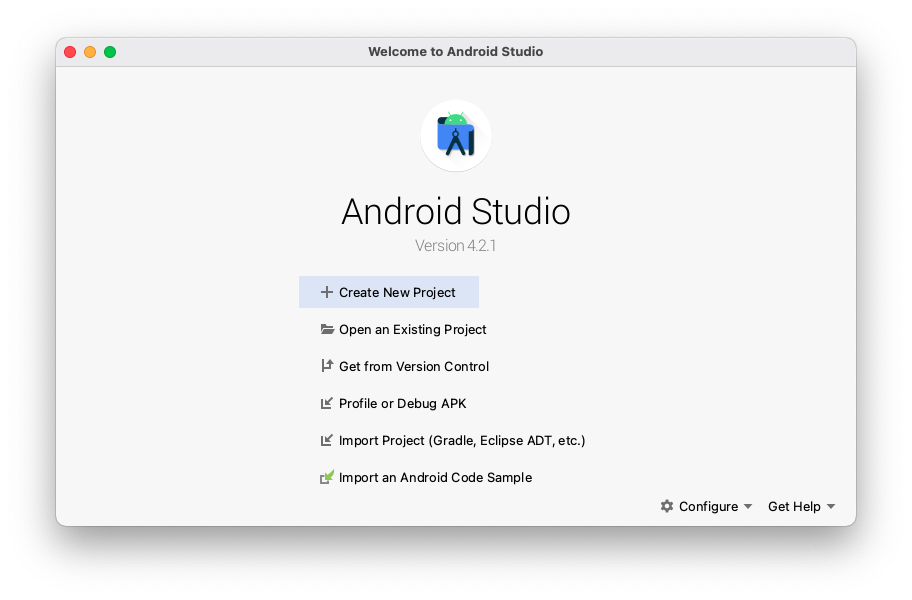
\includegraphics[width=7cm]{img/kmm-start-1} }}
    
    \subfloat[\centering Nieuw project met de KMM application optie]{{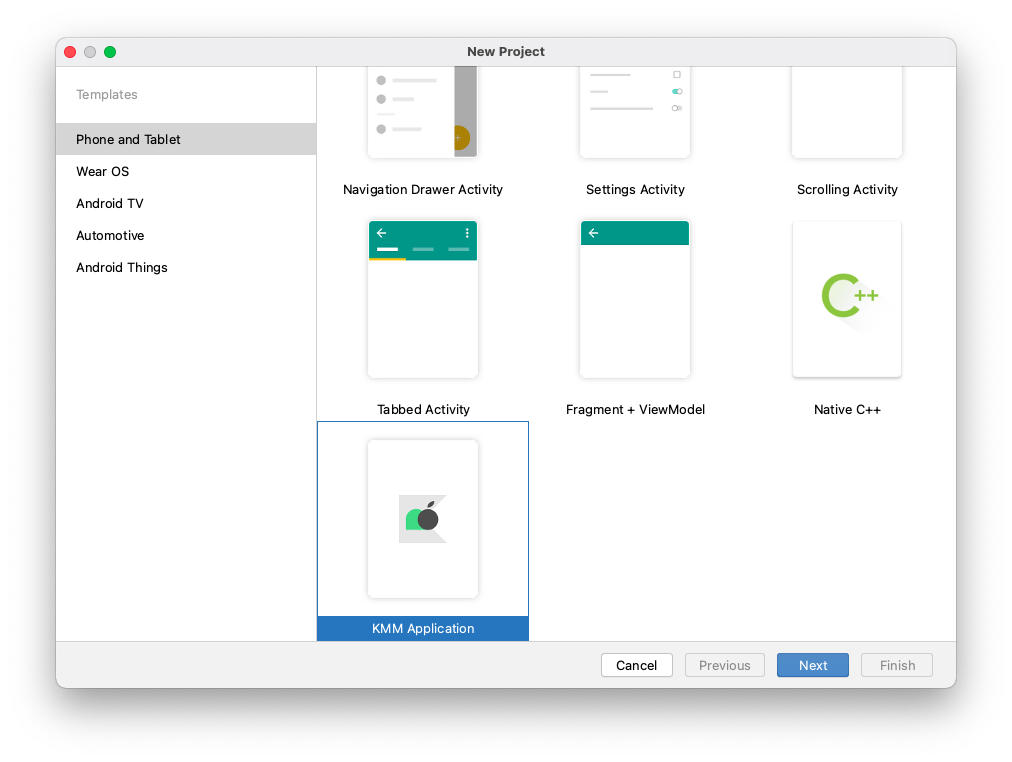
\includegraphics[width=7cm]{img/kmm-start-2} }}
    
    \subfloat[\centering Standaard instellingen Android Project]{{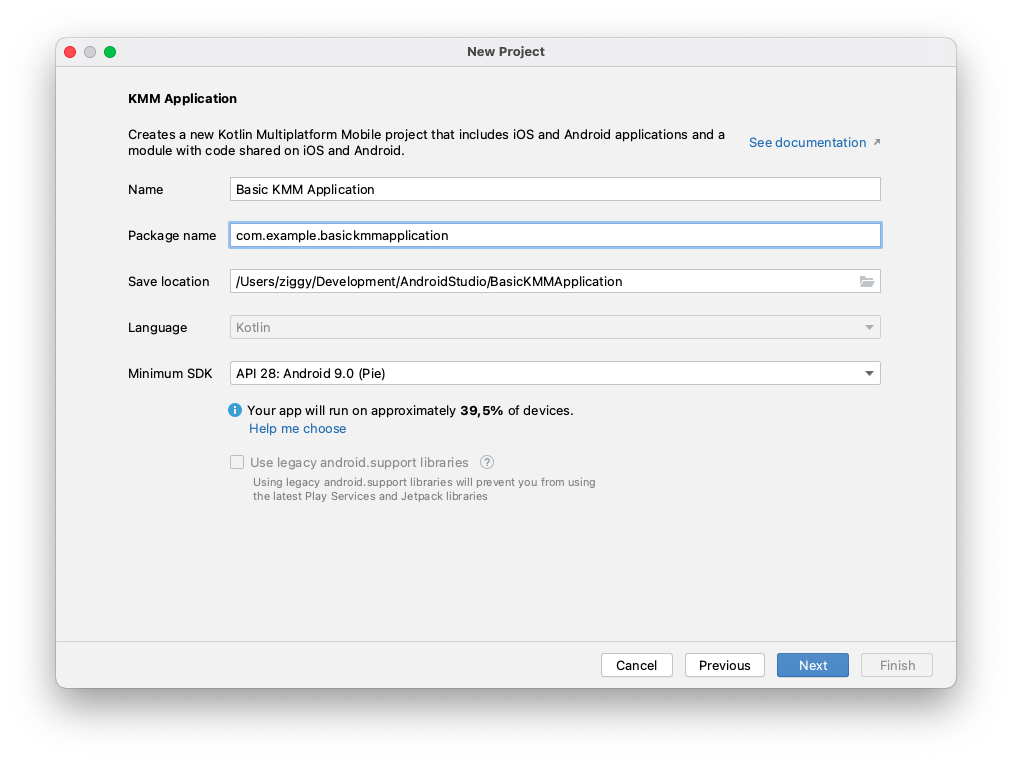
\includegraphics[width=7cm]{img/kmm-start-3} }}
    
    \subfloat[\centering Specifieke KMM project instellingen]{{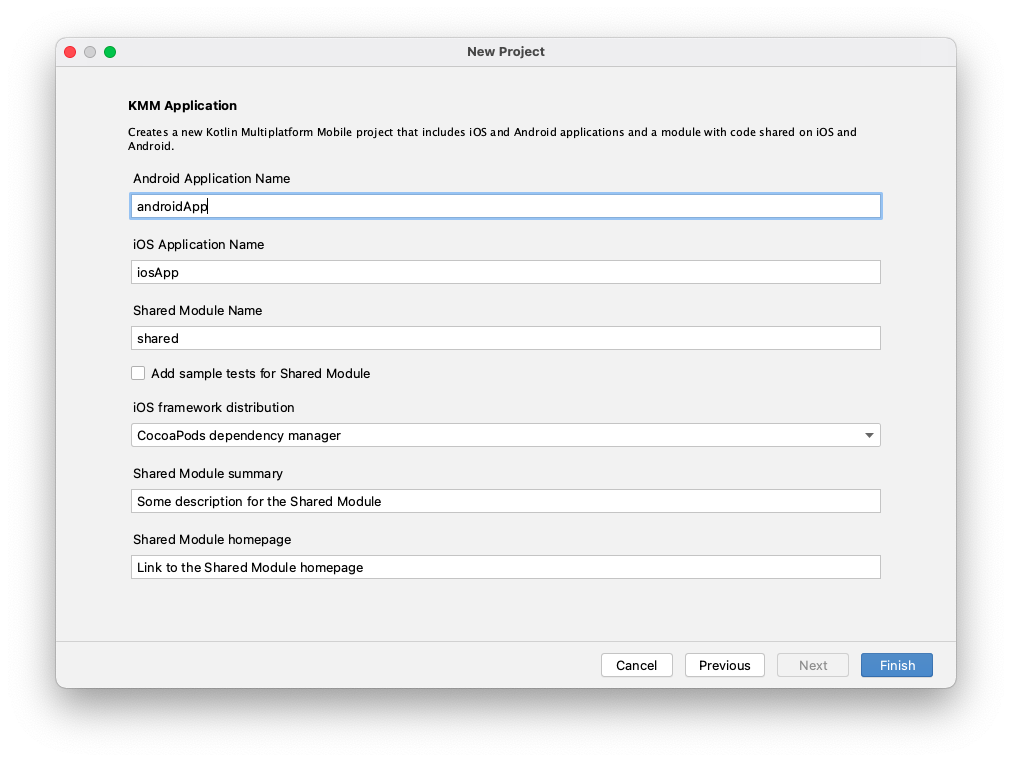
\includegraphics[width=7cm]{img/kmm-start-4} }}
    \caption{Proces voor het opzetten van een KMM project}
    \label{fig:M-kmm-startup}
\end{figure}

Eens het project correct is ingeladen en geïndexeerd, kan gezien worden dat het project al standaard de code bevat om een gebruiker zijn software versie te tonen. Daarnaast zal de KMM plugin binnen Android Studio de juiste omgevingen aanmaken om de code te draaien/testen binnen de juiste emulators. 

\begin{figure}
    \centering
    \subfloat[\centering Instellingen Android emulator]{{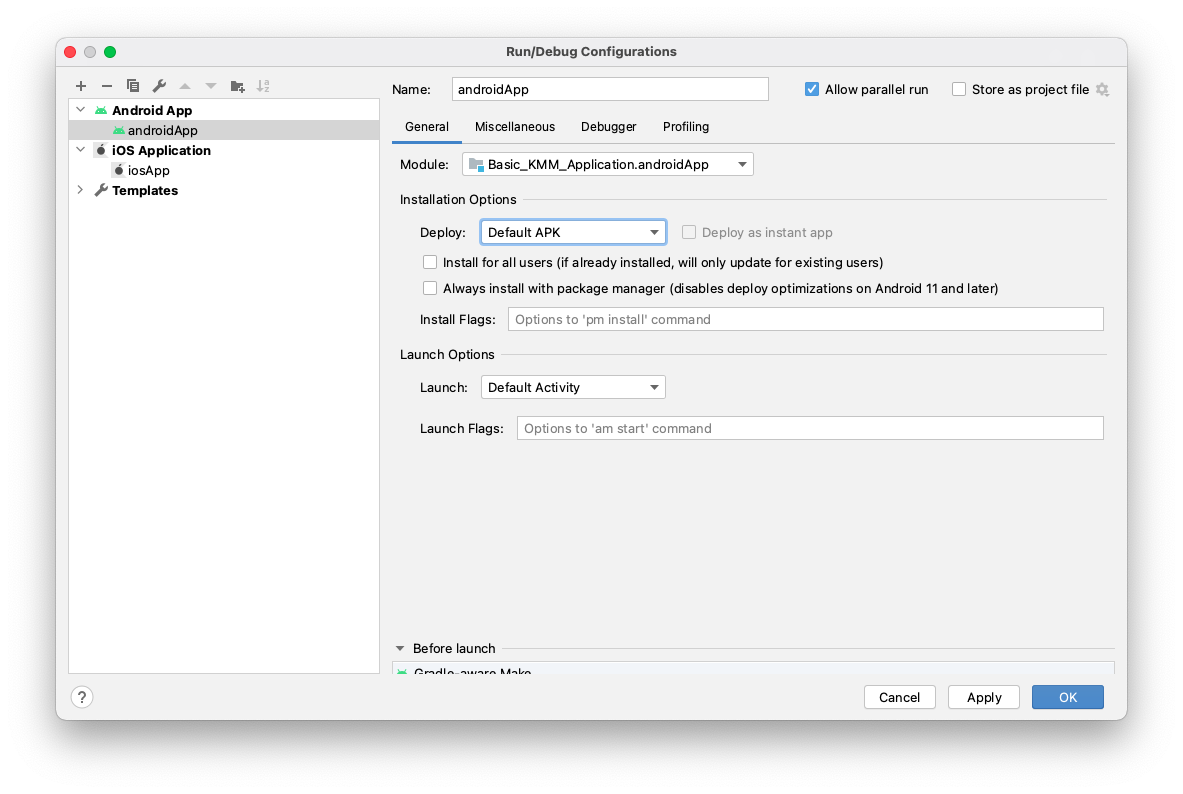
\includegraphics[width=8cm]{img/as-emulators-1} }}
    
    \subfloat[\centering Instellingen iOS emulator]{{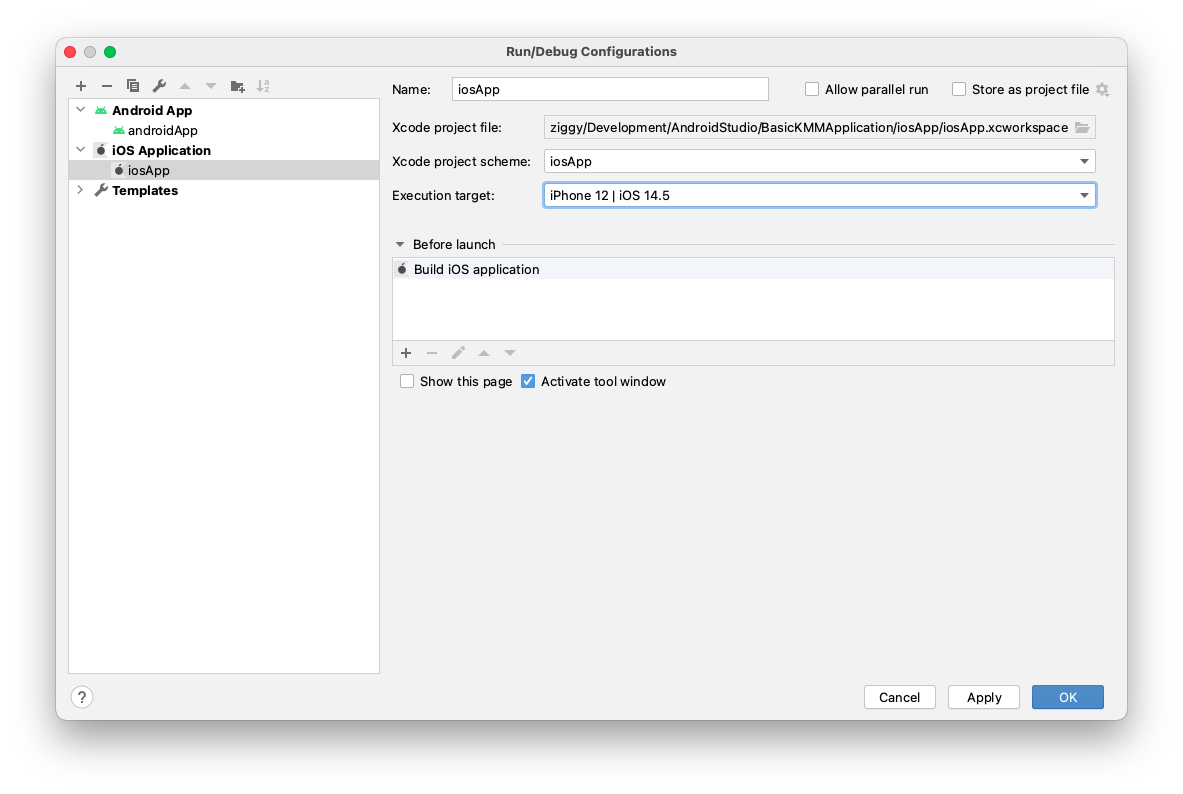
\includegraphics[width=8cm]{img/as-emulators-2} }}
    
    \caption{Android en iOS emulators binnen Android Studio}
    \label{fig:M-as-emulators}
\end{figure}

Eens de emulators ingesteld zijn, kan het project voor iOS en Android worden opgestart. Na 8s 8374ms was de Android applicatie voor de eerste keer opgestart en na 6s 202ms was de iOS applicatie opgestart. Hieronder een beeld van beide applicaties in actie.

\begin{figure}
    \centering
    \subfloat[\centering Android applicatie]{{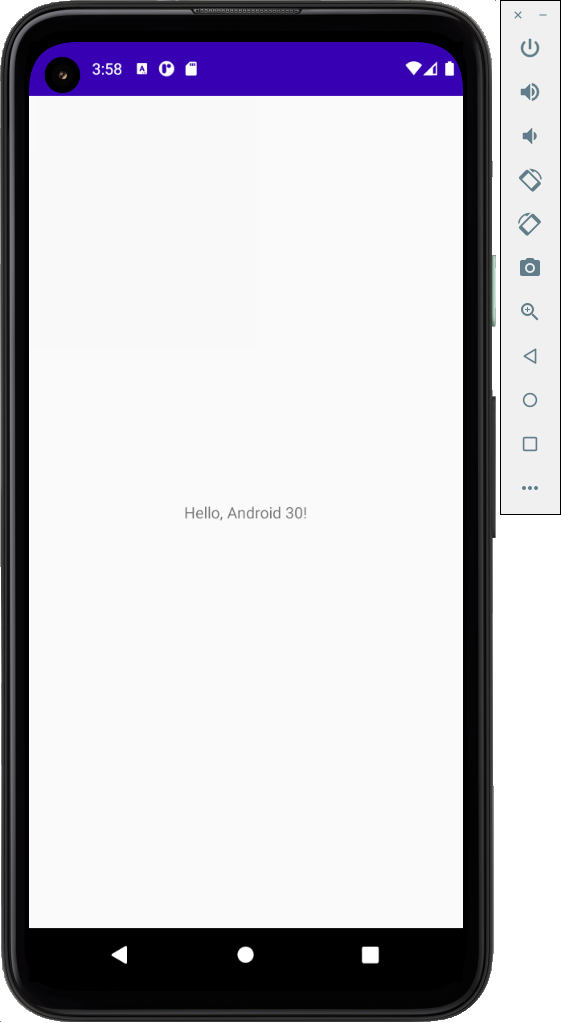
\includegraphics[width=4cm]{img/kmm-basic-android} }}
    \qquad
    \subfloat[\centering iOS applicatie]{{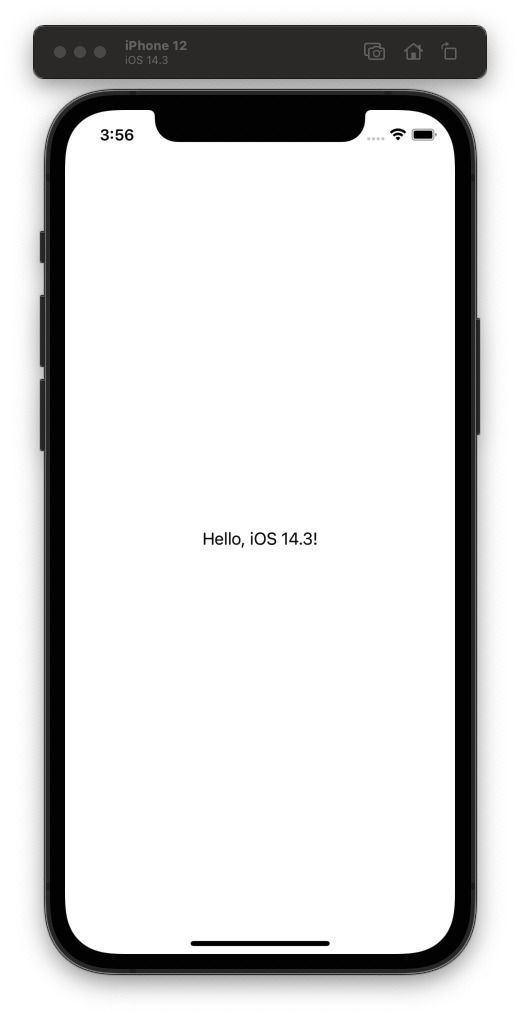
\includegraphics[width=4cm]{img/kmm-basic-ios} }}
    \caption{KMM basic applicatie op Android en iOS}
    \label{fig:M-kmm-basic}
\end{figure}

\begin{figure}
    \centering
    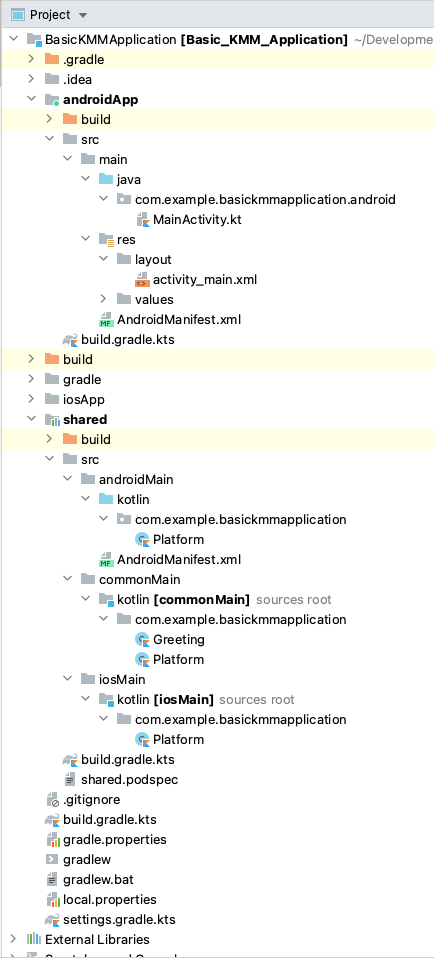
\includegraphics[width=7cm]{img/kmm-structure.png}
    \caption{Projectstructuur van het KMM project}
    \label{fig:M-kmm-stucture}
\end{figure}

Binnen het project kan de expect/actual structuur duidelijk teruggevonden worden. Binnen de shared-map, die te zien is op figuur \ref{fig:M-kmm-stucture}, bevindt zich de commonMain-map. Hierin zitten volgende twee bestanden.

\begin{lstlisting}
    //Greeting.kt
    
    class Greeting {
        fun greeting(): String {
            return "Hello, ${Platform().platform}!"
        }
    }
\end{lstlisting}
\begin{lstlisting}
    //Platform.kt
    
    expect class Platform() {
        val platform: String
    }
\end{lstlisting}

Ook in de shared-map kan de iosMain-map gevonden worden. Hierin komt het Platform.kt bestand nogmaals terug. Hierbij wordt echter de `expect' geïmplementeerd en verwerkt in de `actual'. 

\begin{lstlisting}
    //Platform.kt
    
    actual class Platform actual constructor() {
        actual val platform: String = 
            UIDevice.currentDevice.systemName() + 
            " " + 
            UIDevice.currentDevice.systemVersion
    }
\end{lstlisting}

De laatste map binnen de shared-map die interessant is voor deze studie is de androidMain-map en hierin wordt ook de Platform.kt verwerkt.

\begin{lstlisting}
    //Platform.kt
    
    actual class Platform actual constructor() {
        actual val platform: String = 
            "Android ${android.os.Build.VERSION.SDK_INT}"
    }
\end{lstlisting}

Verdere uitleg omtrent de code zal gebeuren in de delen van de native applicaties gezien de code daar hetzelfde is.
\\ \\ 
Zoals duidelijk zichtbaar zal in de shared-map de globale structuur worden vastgelegd en deze zal dan verwerkt worden binnen de platform specifieke delen.
\\ \\ 
Uiteindelijk zal de Greetings klasse worden opgeroepen binnen de Android en iOS applicaties zoals hieronder geïllustreerd.
\begin{lstlisting}
    //Android - MainActivity.kt
    
    fun greet(): String {
        return Greeting().greeting()
    }
\end{lstlisting}
\begin{lstlisting}
    //iOS - ContentView.swift
    
    struct ContentView: View {
       let greet = Greeting().greeting()
       
       var body: some View {
           Text(greet)
       }
    }
   
\end{lstlisting}

\section{\IfLanguageName{dutch}{Basis native applicaties}{Basic native applications}}
\label{sec:M-first-native}
Nu de KMM applicatie gemaakt is, kan de native variant voor Android en iOS gemaakt worden. Hierbij zal geprobeerd worden deze zo goed mogelijk op elkaar af te stemmen.
\\ \\
De geschreven applicaties kunnen ook op GitHub\footnote{github.com} teruggevonden worden. Dit kan via volgende links:
\\ \\
\textbf{Android}:
\\
\verb*|https://github.com/ziggymoens/Android_Native_Basic|
\\ \\
\textbf{iOS}:
\\
\verb*|https://github.com/ziggymoens/iOS_Native_Basic|
\\ \\

\subsection{\IfLanguageName{dutch}{Android}{Android}}
\label{sec:M-first-native-android}
Het eerste native project dat gemaakt zal worden is het Android project. Dit project zal ook geschreven worden in Kotlin binnen Android Studio. Bij het aanmaken van een nieuw project kan de optie 'Empty Activity' gekozen worden. Daarna worden volgende gegevens ingevuld, te zien of figuur \ref{fig:M-basic-android-start}. Voor de layout worden de AndroidX\footnote{developer.android.com/jetpack/androidx} bibliotheken gebruikt.

 \begin{figure}
    \centering
    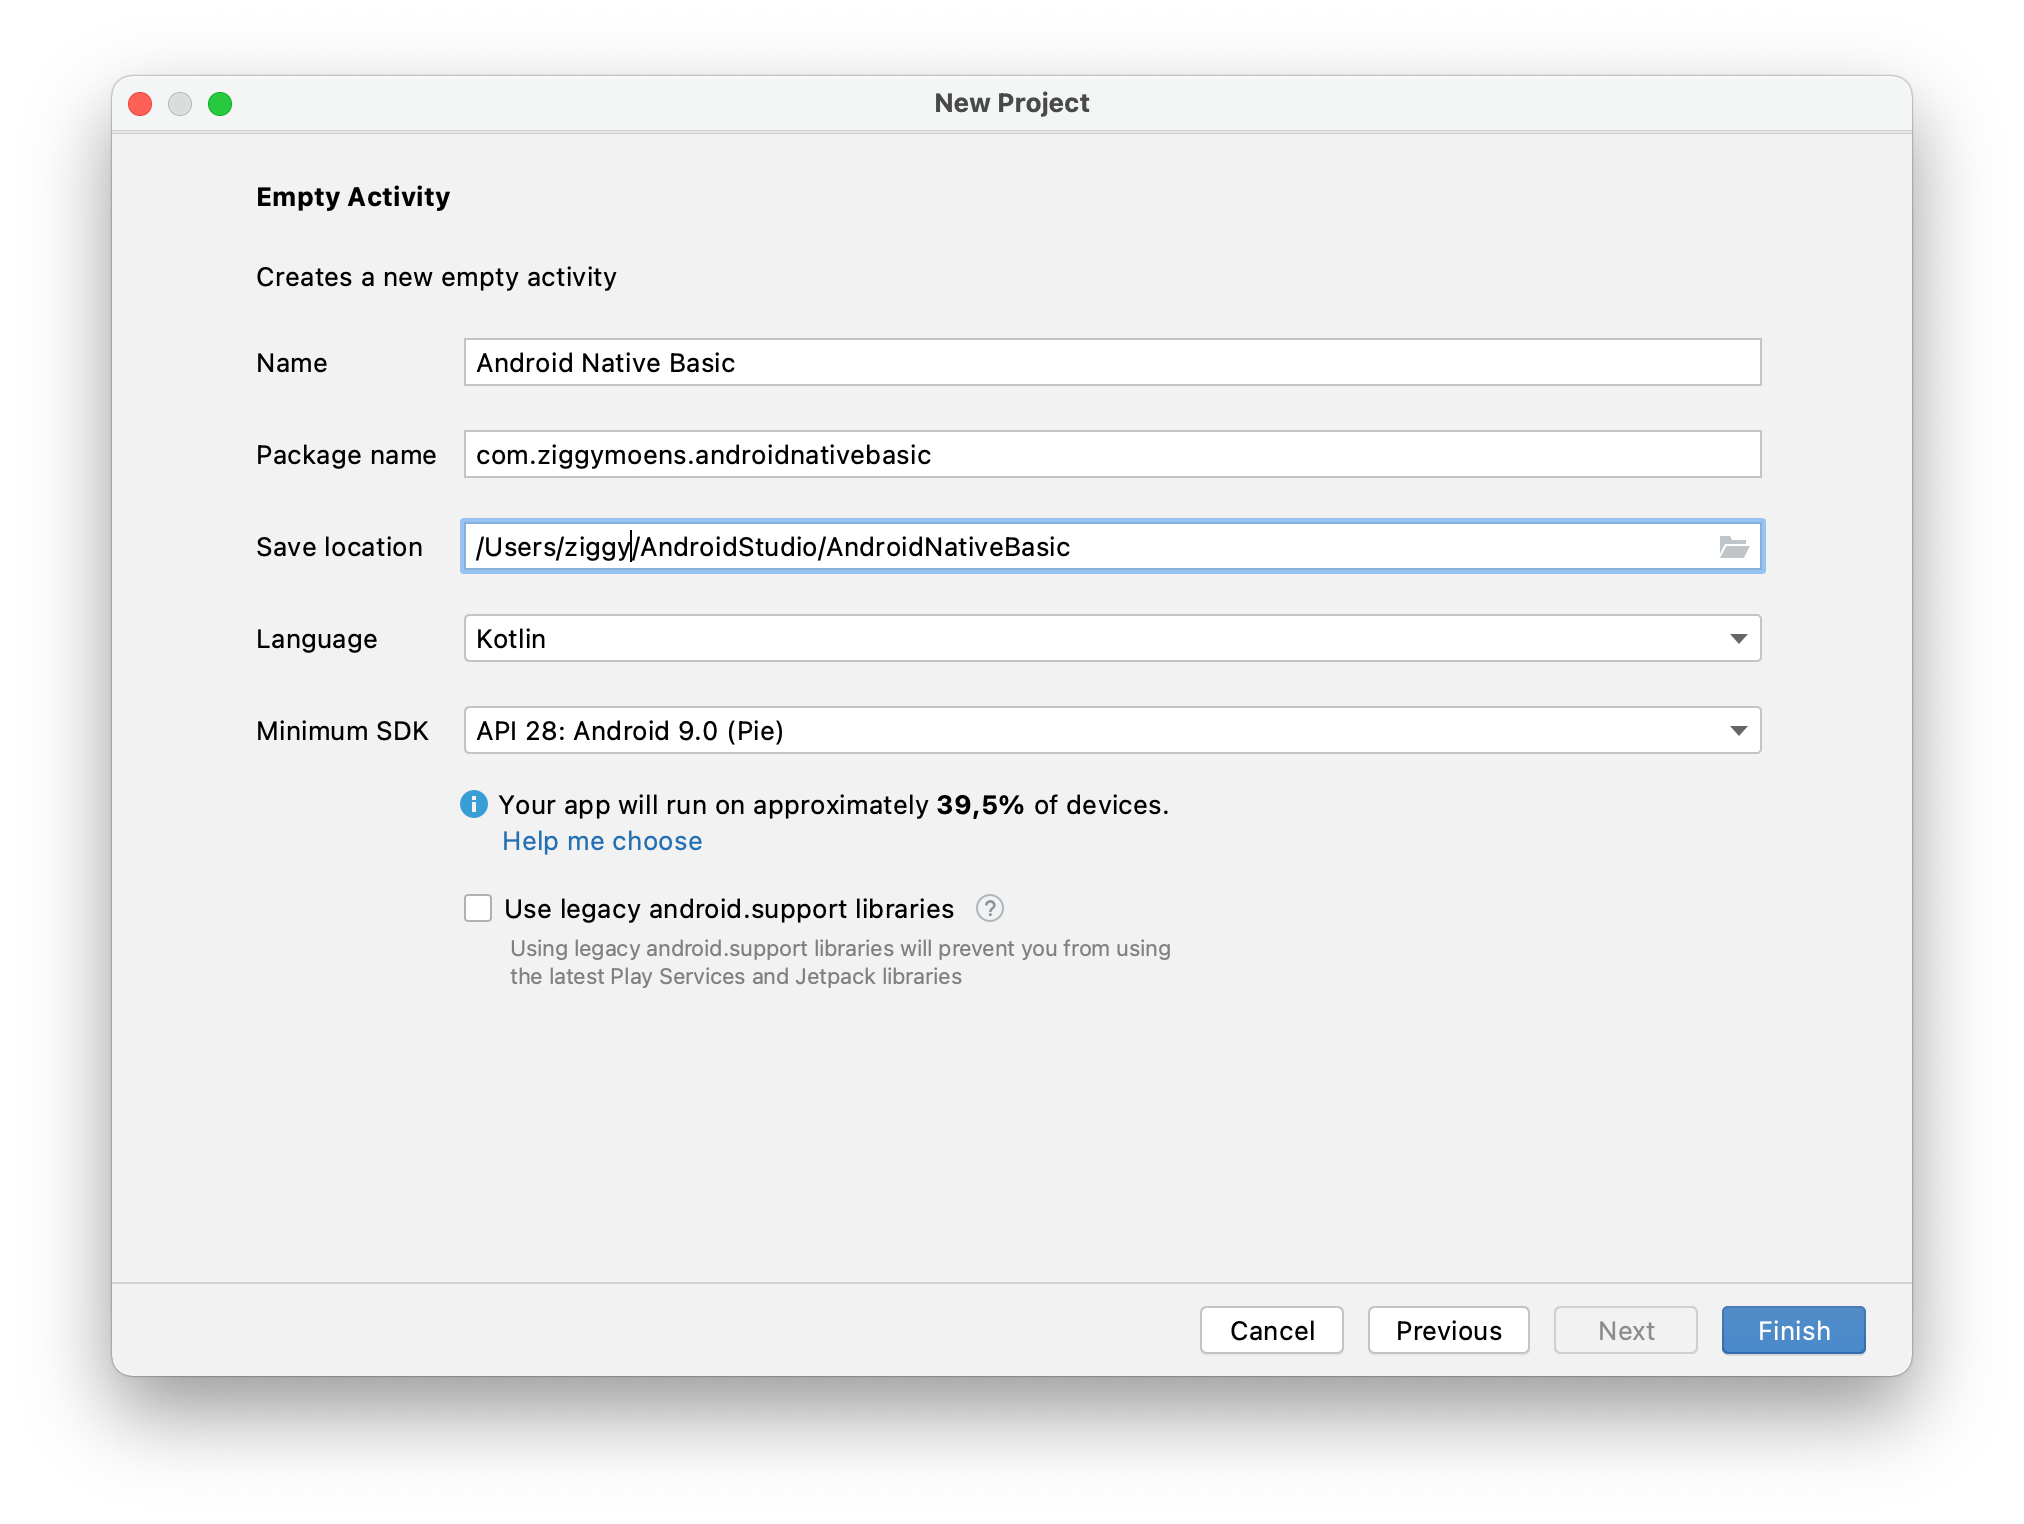
\includegraphics[width=14cm]{img/android-basic-start.png}
    \caption{Instelling voor het native Android project}
    \label{fig:M-basic-android-start}
\end{figure}

Eens het project is geïndexeerd en Gradle\footnote{gradle.org} voor de eerste keer alles heeft gebuild, kan gestart worden met de ontwikkeling van de applicatie. Hierbij zijn er twee zaken die moeten gebeuren: 
\begin{itemize}
    \item Het invullen van de MainActivity zodat de juiste versie van Android getoond wordt aan de gebruiker
    \item Het aanmaken van een layout file zodat ook de user interface overeenstemt met de KMM applicatie
\end{itemize}

Binnen de Main Activity kan `android.os.Bundle' geïmporteerd worden, via deze weg kan achterhaald worden wat de huidige Android versie van het betreffende toestel is. Deze waarde zal een getal teruggeven en binnen de gecontroleerde omgeving van de emulator wordt hier versie 30 verwacht.
\\ \\
Voor de Main Activity is de code als volgt:

\begin{lstlisting}
    //MainActivity.kt
    class MainActivity : AppCompatActivity() {
        
        override fun onCreate(savedInstanceState: Bundle?) {
            super.onCreate(savedInstanceState)
            setContentView(R.layout.activity_main)
            
            val tv: TextView = findViewById(R.id.text_view)
            tv.text = "Hello, Android ${android.os.Build.VERSION.SDK_INT}!"
        }
    }
\end{lstlisting}

Binnen de layout file wordt enkel een tekstveld geplaatst met het id `text\_view', zodat deze binnen de Main Activity kan worden opgeroepen. Daarnaast wordt het tekstveld horizontaal en verticaal gecentreerd binnen het scherm, dit gebeurt aan de hand van een ConstraintLayout\footnote{developer.android.com/training/constraint-layout}.
\\ \\ 
Voor de layout file wordt volgende code bekomen:

\begin{lstlisting}
    //activity_main.xml
    <?xml version="1.0" encoding="utf-8"?>
    <androidx.constraintlayout.widget.ConstraintLayout xmlns:android="http://schemas.android.com/apk/res/android"
       xmlns:app="http://schemas.android.com/apk/res-auto"
       xmlns:tools="http://schemas.android.com/tools"
       android:id="@+id/main_view"
       android:layout_width="match_parent"
       android:layout_height="match_parent">
    
       <TextView
           android:id="@+id/text_view"
           android:layout_width="wrap_content"
           android:layout_height="wrap_content"
           app:layout_constraintBottom_toBottomOf="parent"
           app:layout_constraintLeft_toLeftOf="parent"
           app:layout_constraintRight_toRightOf="parent"
           app:layout_constraintTop_toTopOf="parent"
           tools:text="Hello World!" />
                
    </androidx.constraintlayout.widget.ConstraintLayout>
\end{lstlisting}

Eens de code geschreven is kan deze voor een eerste maal uitgevoerd worden op de emulator. Figuur \ref{fig:M-basic-android} toont de user interface van de Android applicatie.

\begin{figure}
    \centering
    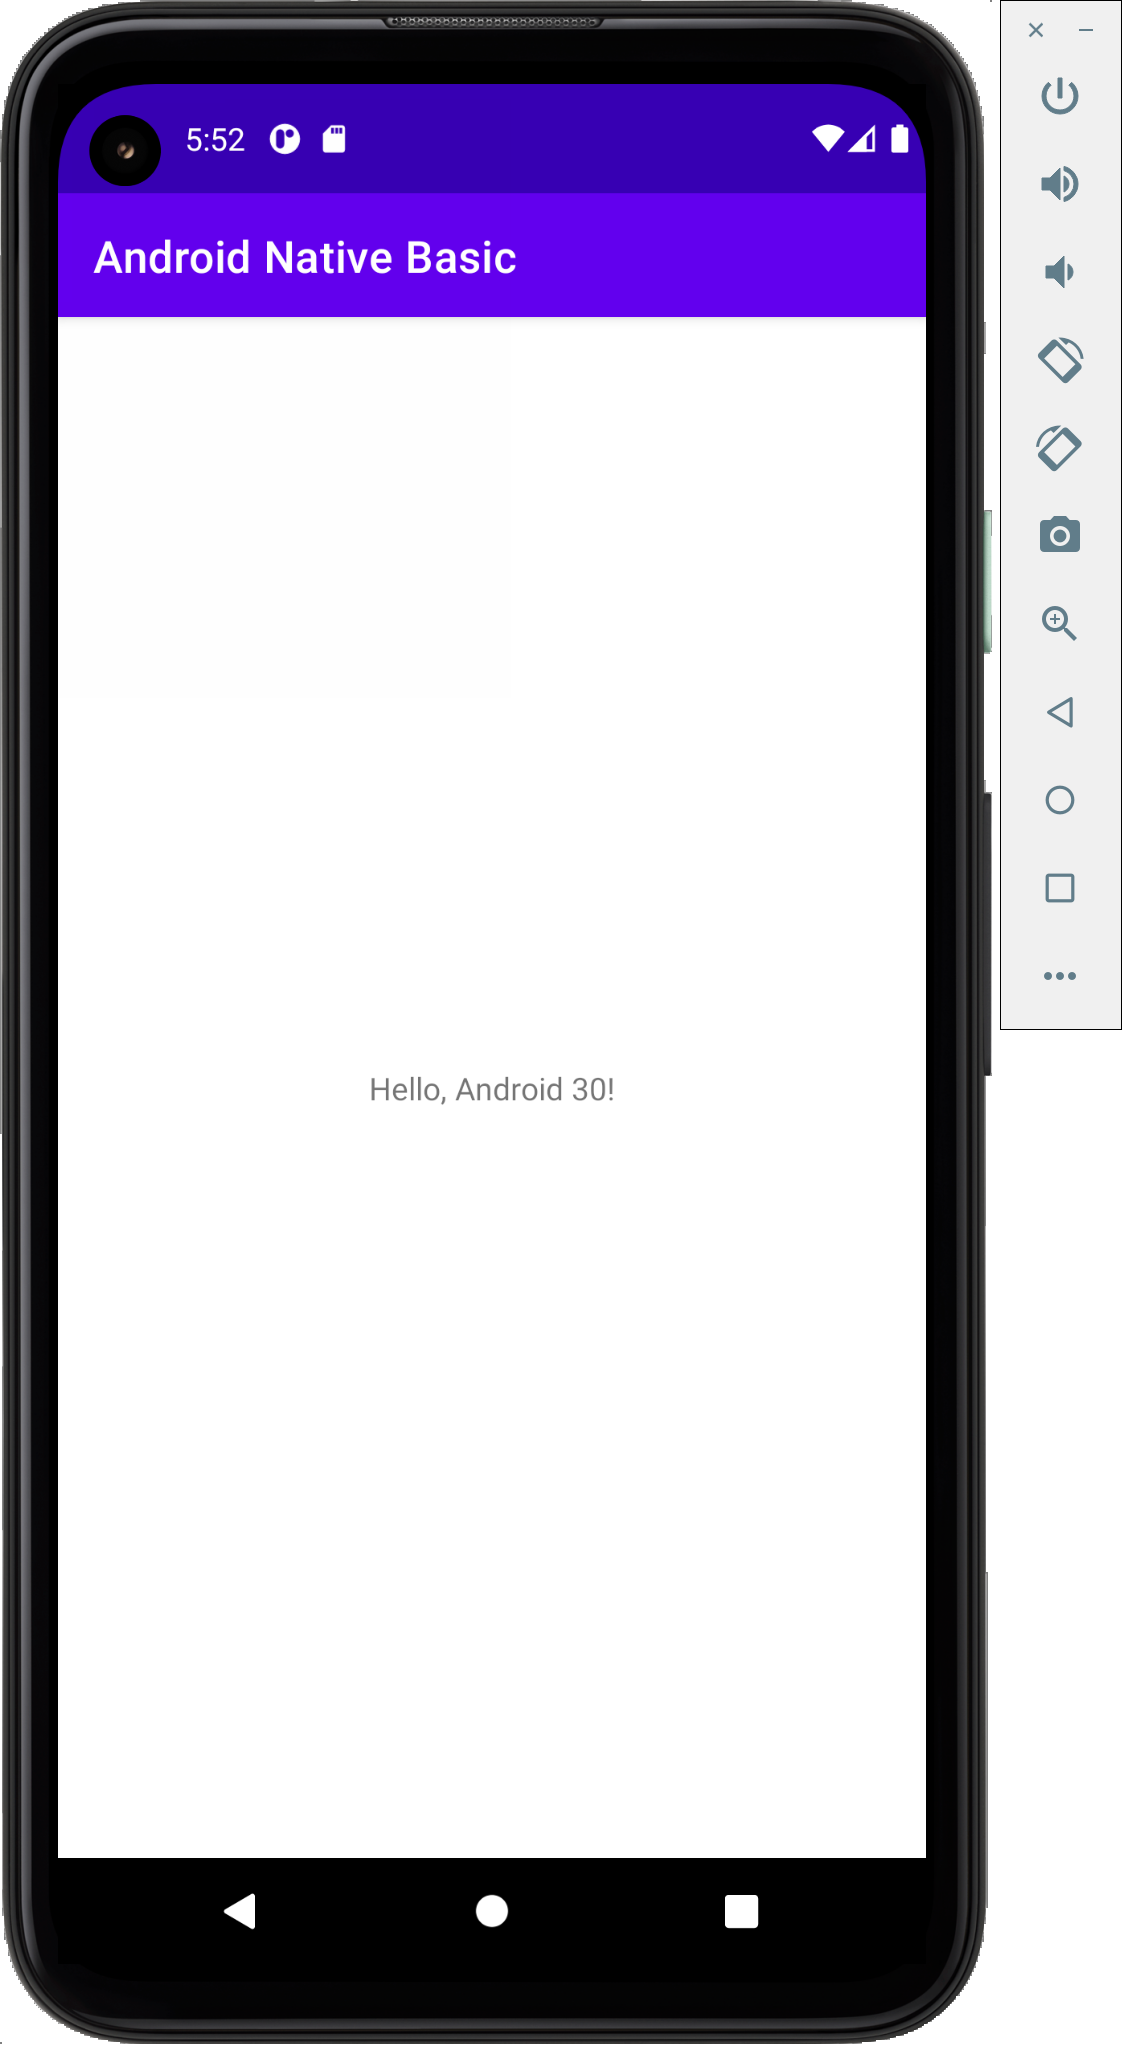
\includegraphics[width=7cm]{img/android-basic.png}
    \caption{Interface van de basic native Android applicatie}
    \label{fig:M-basic-android}
\end{figure}

\subsection{\IfLanguageName{dutch}{iOS}{iOS}}
\label{sec:M-first-native-ios}
De andere native applicatie die dient geschreven te worden is een iOS applicatie. Deze applicatie zal geschreven worden in Swift\footnote{apple.com/benl/swift} binnen Xcode. Voor deze applicatie zal gebruik gemaakt worden van UIKit\footnote{developer.apple.com/documentation/uikit} voor de layout van de applicatie. Binnen Xcode zal gekozen worden voor een nieuw project namelijk een iOS App.

\begin{figure}
    \centering
    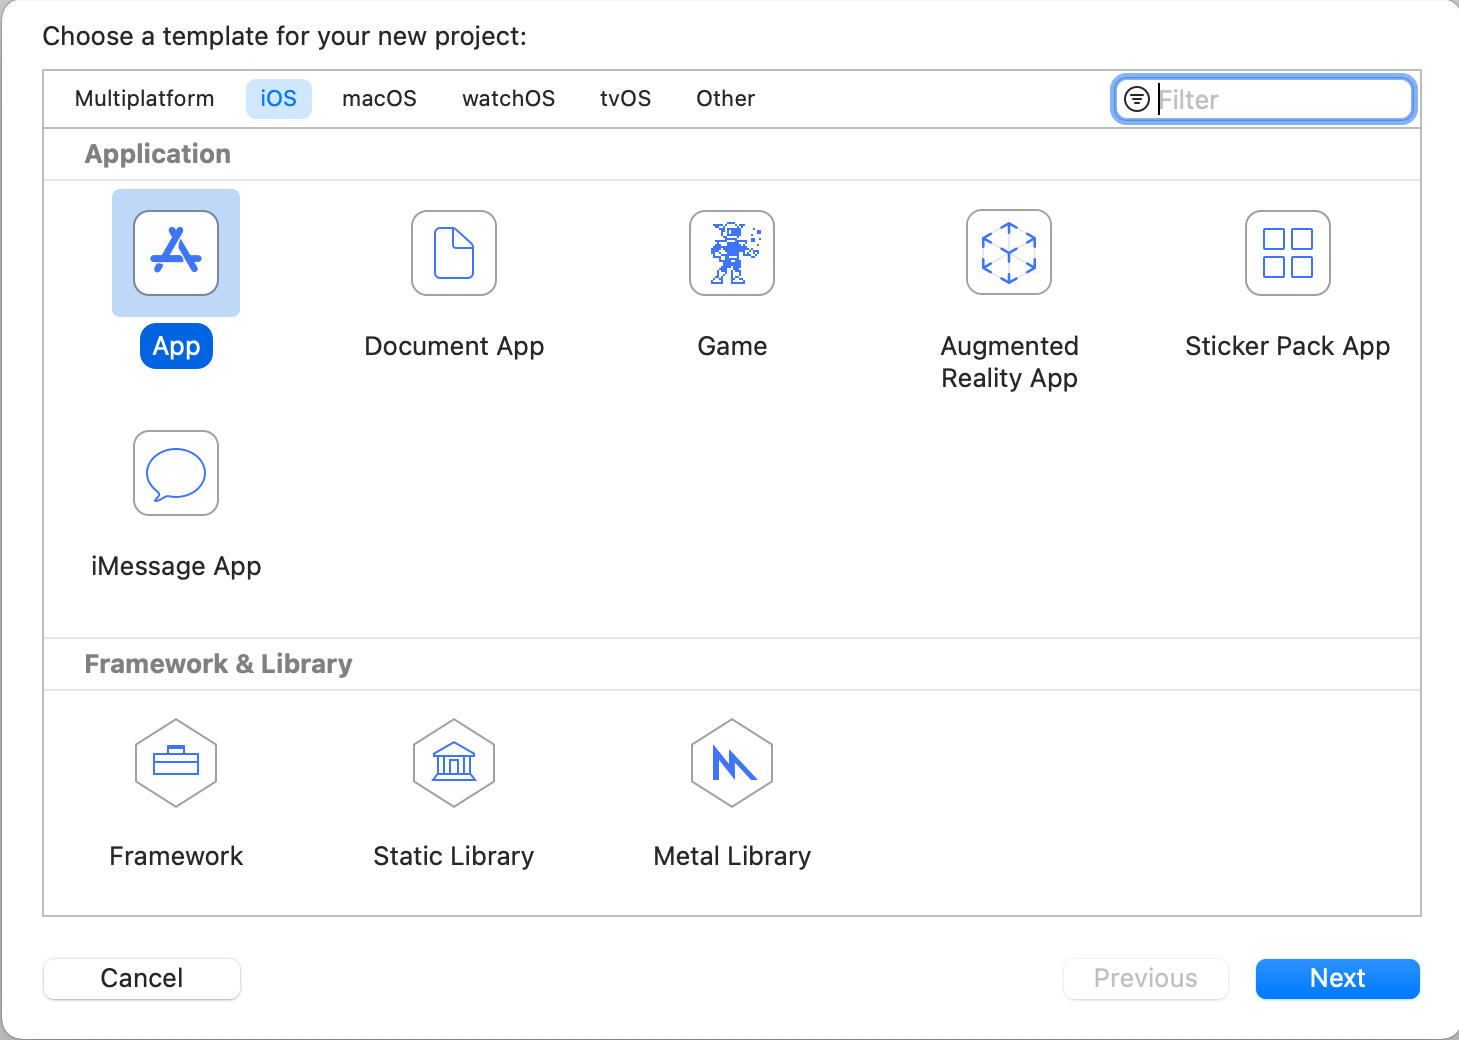
\includegraphics[width=7cm]{img/ios-basic-start.png}
    \caption{De optie voor een nieuwe iOS App binnen Xcode}
    \label{fig:M-basic-ios-start}
\end{figure}

\begin{figure}
    \centering
    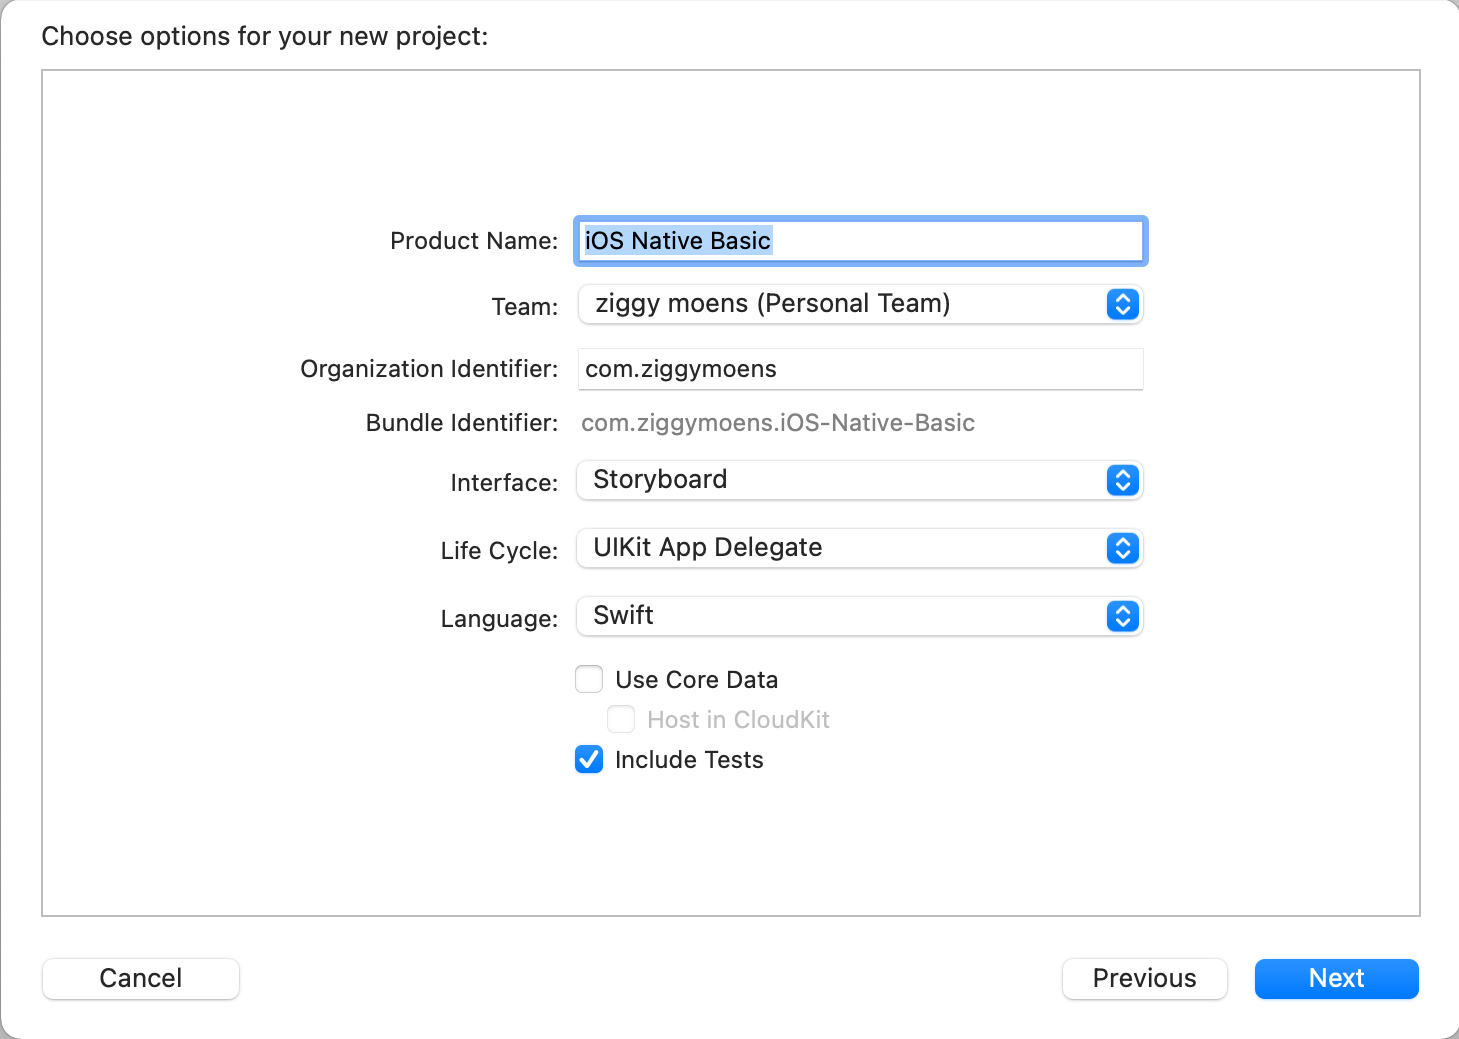
\includegraphics[width=7cm]{img/ios-basic-settings.png}
    \caption{Instelling voor het native iOS project}
    \label{fig:M-basic-ios-settings}
\end{figure}

De eerste stap voor het iOS project is het aanmaken van het label in de user interface, dit gebeurt via het Storyboard. Daarna kan de link gelegd worden tussen de user interface en de view controller. Binnen de view controller kan daarna de juiste waarde gegeven worden aan het tekstveld. De iOS applicatie kunnen we aan de hand van `UIDevice' de gegevens ophalen van het toestel dat de applicatie aan het draaien is. UIDevice is een deel van het UIKit framework en zit standaard geïmplementeerd in de view controllers.

Uiteindelijk wordt volgende code voor de view controller bekomen: 
\begin{lstlisting}
    // ViewController.swift
    
    class ViewController: UIViewController {
        
        @IBOutlet weak var label: UILabel!
        
        override func viewDidLoad() {
            super.viewDidLoad()
            
            label.text = "Hello, " + UIDevice.current.systemName + " " + UIDevice.current.systemVersion
        }
    }
    
\end{lstlisting}

Eens al de code geschreven is kan de code getest worden op de iPhone 12 emulator binnen Xcode. Figuur \ref{fig:M-basic-ios} toont de interface van de basic native iOS applicatie.

\begin{figure}[H]
    \centering
    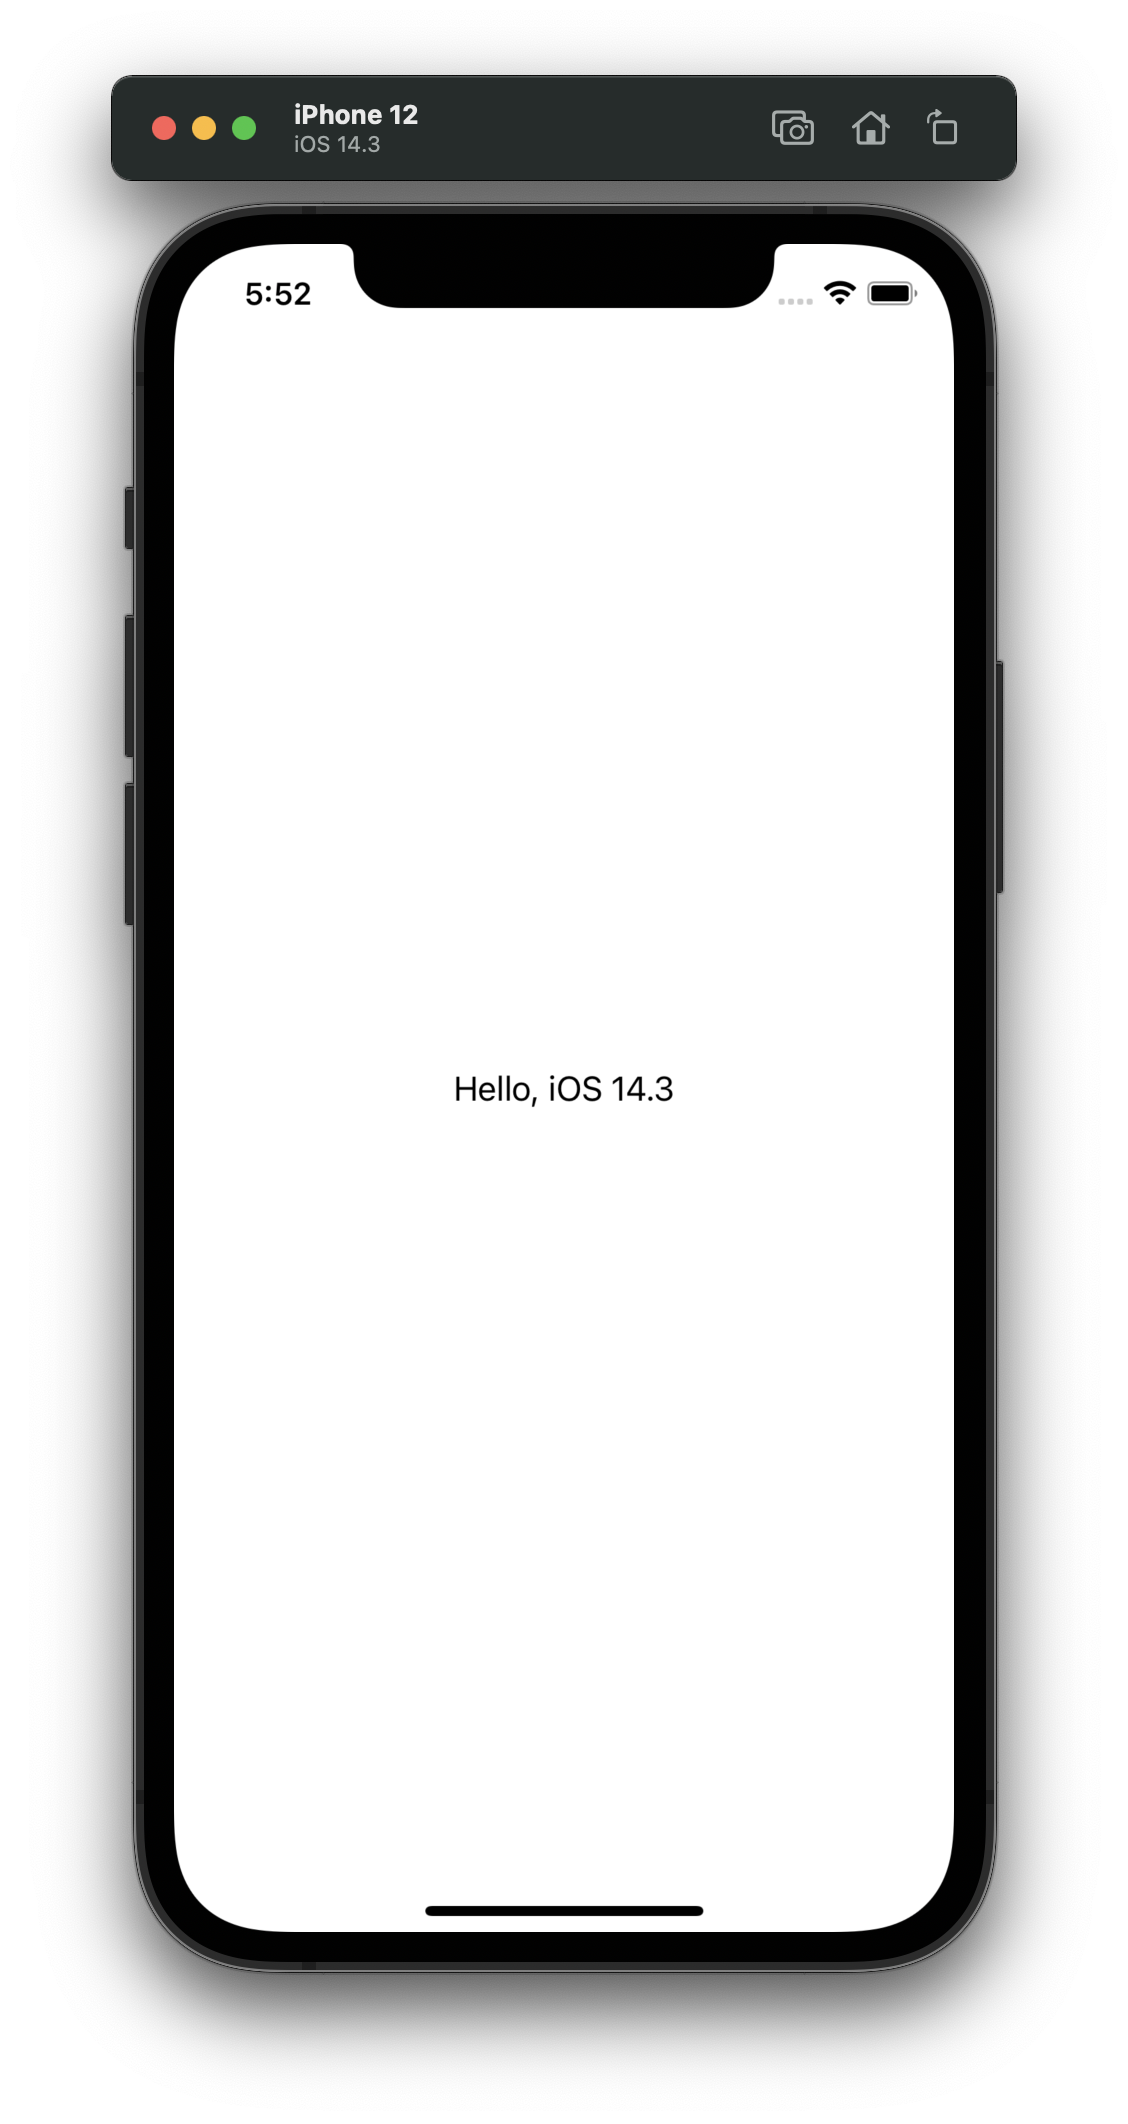
\includegraphics[width=7cm]{img/ios-basic.png}
    \caption{Interface van de basic native iOS applicatie}
    \label{fig:M-basic-ios}
\end{figure}

\section{\IfLanguageName{dutch}{Testen van de basis applicaties}{Testing of the basic applications}}
\label{sec:M-testing-basic}
Gezien de basis applicaties reeds geschreven werden, kan nu overgegaan worden op de testen ervan. Hierbij een overzicht van de uit te voeren testen op de applicaties:

\begin{itemize}
    \item Aantal lijnen code
    \item Compileersnelheid
    \item Voetafdruk
    \item Ontwikkeltijd
    \item Kostprijs
\end{itemize}

\subsection{\IfLanguageName{dutch}{Aantal lijnen code}{Aantal lijnen code}}
\label{sec:M-test-lijnen-code}
De eerste test gaat het aantal lijnen code na. Voor deze test is de Statistics\footnote{https://plugins.jetbrains.com/plugin/4509-statistic} plug-in geïnstalleerd binnen Android studio
\\ \\
De \textbf{Statistics plug-in} kan via volgende link teruggevonden worden:\\
\verb*|https://plugins.jetbrains.com/plugin/4509-statistic|
\\ \\
De instellingen kunnen op volgende plek teruggevonden worden \\ 
\underline{Android Studio -> Voorkeuren -> Tools -> Statistics}
\\ \\
Voor deze testen worden volgende specifieke instellingen geselecteerd: \\
\underline{Excluded file types}:\\ `class;svn-base;svn-work;Extra;gif;png;jpg;jpeg;bmp;tga;tiff;ear;war;zip;jar;iml;iws;ipr;bz2;gz;pyc;'
\underline{Seperate TABs file types:}\\
`java;xml;css;html;js;properties;jsp;txt;php;php4;php5;phtml;inc;py;vue;kt'
\\ \\
Daarnaast dienen volgende opties aangevinkt te worden:\\
\begin{itemize}
    \item Exclude compiler output directory
    \item Exclude IDEA9+ artifact directory (.idea)
    \item Exclude NPM directory (node\_modules)
    \item Exclude PyCache directory (\_\_pycache\_\_)
    \item Exclude Git directory (.git)
    \item Exclude Subversion directory (.svn)
    \item Exclude Android (R.java)
    \item Exclude Minified Javascript (*.min.js)
    \item Exclude Minified StyleSheet (*.min.css)
    \item Exclude all directories starting with (.)
    \item Exclude MAVEN output directories (target)
\end{itemize}

Figuur \ref{fig:M-test-lijnen-code-settings} toont de instellingen binnen Android Studio.
\begin{figure}[h!]
    \centering
    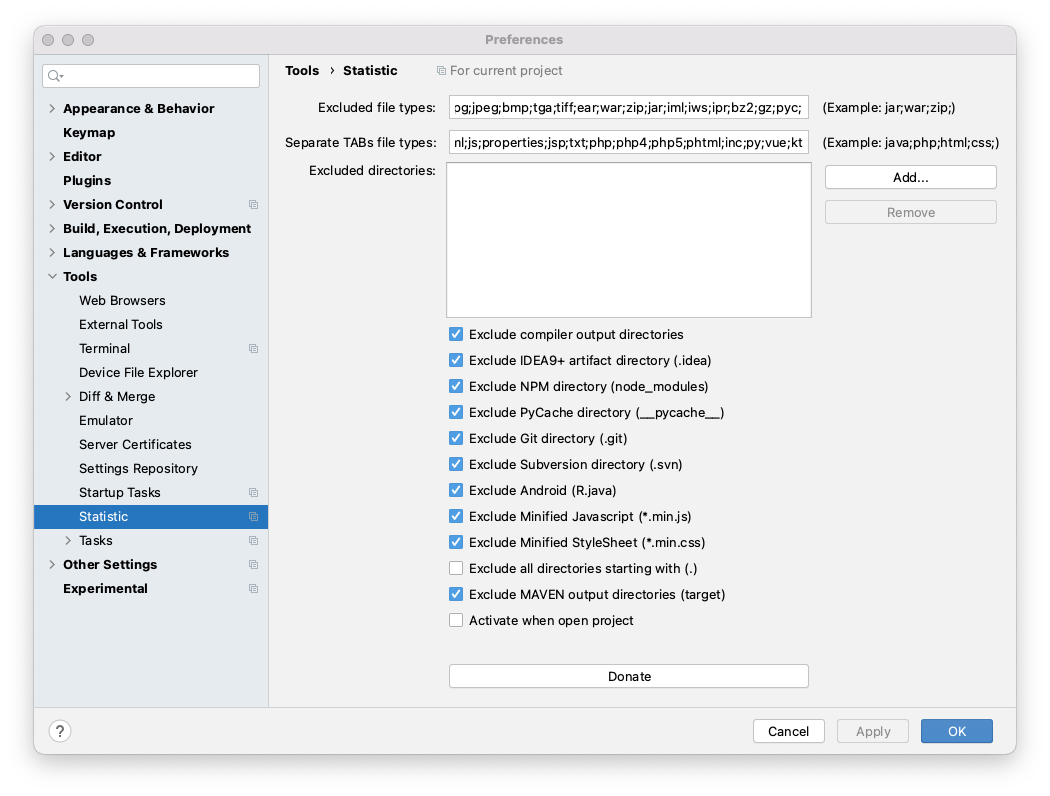
\includegraphics[width=10cm]{img/statistics-settings.png}
    \caption{Instellingen voor de Statics plug-in}
    \label{fig:M-test-lijnen-code-settings}
\end{figure}


Voor de projecten zal dezelfde plug-in en IDE gebruikt worden. Hierdoor kunnen fouten in de meting tot een minimum beperkt worden. Voor de gedetailleerde resultaten wordt verwezen naar bijlage \ref{ch:results-code} `Resultaten van aantal lijnen code'.

In tabel \ref{T:lines-overzicht} staat de samenvatting van resultaten de drie projecten. Het iOS werd, net zoals Android en KMM, ingeladen in Android Studio zodat de Statistics plug-in gebruikt kon worden.

\begin{table}[H]
    \centering
    \caption{Statistiek resultaten voor KMM en de native projecten}
    \begin{tabular}{|l|c|c|c|}
        \hline
        {\textbf{Factor}} & {\textbf{iOS}} &\textbf{Android} &\textbf{KMM} \\ \hline \hline
        Aantal bestanden&18&20&41\\ \hline
        Totale grote&90649 B&17906 B&77725 B\\ \hline
        Kleinste bestand&75691 B&3745 B&42370 B\\ \hline
        Grootste bestand&82640 B&10466 B&54864 B\\ \hline
        Gemiddelde grootte&78547 B&5322 B&48330 B\\ \hline
        Aantal lijnen&1857&495&1779\\ \hline
        Lijnen code&1634&389&1605\\ \hline
    \end{tabular}
    \label{T:lines-overzicht}
\end{table}

\subsubsection{\IfLanguageName{dutch}{Conclusie}{Conclusion}}
\label{sec:M-test-lijnen-code-conclusion}
Uit deze resultaten kunnen enkele conclusies getrokken worden.
\begin{itemize}
    \item Het KMM platform bevat niet meer lijnen code dan native Android en iOS samen\\
    \underline{KMM:} 1605 lijnen\\
    \underline{Native Android + native iOS:} 2023 lijnen\\
    \item Het iOS project is groter, zowel lijnen als omvang, dan het KMM project\\
    \underline{KMM:} 1605 lijnen en 77725 B\\
    \underline{iOS:} 1634 lijnen en 90649 B\\
    \item De Native Android applicatie uitzonderlijk veel kleiner is dan het iOS project\\
    \underline{Android:} 389 lijnen en 17906 B\\
    \underline{iOS:} 1634 lijnen en 90649 B
\end{itemize}

Dit zijn enkele van de meest opvallende en daarnaast ook de meest relevante zaken voor dit onderzoek.

\subsection{\IfLanguageName{dutch}{Compileersnelheid}{Build snelheid}}
\label{sec:M-test-compileersnelheid}
Deze volgende test die werd uitgevoerd is de compileersnelheid test. Hiervoor zal elke applicatie meermaals gecompileerd worden. Hierbij werd geëvalueerd welke applicaties het snelste compileren en dus het meest efficiënt zijn.
\\ \\
Tijdens deze test zullen de basic KMM, Android en iOS applicaties 100 maal gebuild worden. De KMM applicatie werd gebuild in Android Studio (AS) en Xcode. De gedetailleerde resultaten kunnen in deel \ref{ch:results-builds}. De resultaten worden opgesplitst in twee delen namelijk de eerste build en de andere builds. Hierdoor wordt er rekening gehouden met de cache van de IDE.

\subsubsection{\IfLanguageName{dutch}{Eerste compilatie}{First compilation}}
\label{sec:M-test-1-comp}
Tabel \ref{T:1e-compile} toont de resultaten van de eerste compilatie van de applicaties. Hierbij kan worden opgemerkt dat KMM significant sneller is dan native Android en iOS, zeker wetende dat KMM automatisch gebuild is voor beide varianten. De eerste builds bevatten nog geen cache in de IDE dus de performantie is puur afhankelijk van het framework en hoe efficiënt dit werkt. Uit deze resultaten kan dus geconcludeerd worden dat voor deze studie KMM sneller was dan de native varianten.

\begin{table}[H]
    \centering
    \caption{Resulaten van de statistiek voor het KMM project}
    \begin{tabular}{|l|c|}
        \hline
        {\textbf{Platform}} & {\textbf{Eerste compileertijd}} \\ \hline \hline
        Native Android&10,900\\ \hline
        Native iOS&21,531\\ \hline
        KMM - AS&5,873\\ \hline
        KMM - Xcode &10,900\\ \hline
    \end{tabular}
    \label{T:1e-compile}
\end{table}



\subsubsection{\IfLanguageName{dutch}{Andere compilaties}{Other compilations}}
\label{sec:M-test-andere-comp}


Grafiek \ref{G:tijd} toont de resultaten voor de drie applicaties voor compilatie twee tot en met 100:
\\ \\ 
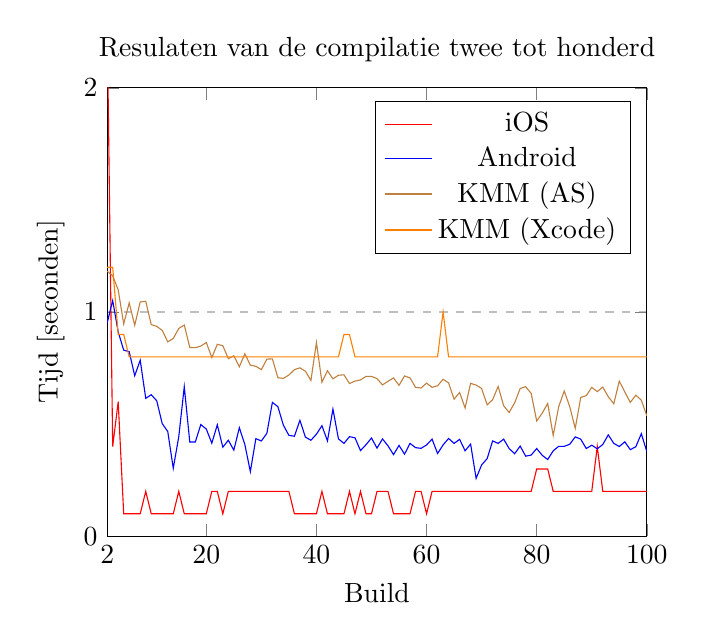
\begin{tikzpicture}
    \begin{axis}[
        title={Resulaten van de compilatie twee tot honderd},
        xlabel={Build},
        ylabel={Tijd [seconden]},
        xmin=2, xmax=100,
        ymin=0, ymax=2,
        xtick={2,20,40,60,80,100},
        ytick={0,1,2},
        legend pos=north east,
        ymajorgrids=true,
        grid style=dashed,
        ]
        
        \addplot[
        color=red
        ]
        coordinates {
            (2,2.300)
            (3,0.400)
            (4,0.600)
            (5,0.100)
            (6,0.100)
            (7,0.100)
            (8,0.100)
            (9,0.200)
            (10,0.100)
            (11,0.100)
            (12,0.100)
            (13,0.100)
            (14,0.100)
            (15,0.200)
            (16,0.100)
            (17,0.100)
            (18,0.100)
            (19,0.100)
            (20,0.100)
            (21,0.200)
            (22,0.200)
            (23,0.100)
            (24,0.200)
            (25,0.200)
            (26,0.200)
            (27,0.200)
            (28,0.200)
            (29,0.200)
            (30,0.200)
            (31,0.200)
            (32,0.200)
            (33,0.200)
            (34,0.200)
            (35,0.200)
            (36,0.100)
            (37,0.100)
            (38,0.100)
            (39,0.100)
            (40,0.100)
            (41,0.200)
            (42,0.100)
            (43,0.100)
            (44,0.100)
            (45,0.100)
            (46,0.200)
            (47,0.100)
            (48,0.200)
            (49,0.100)
            (50,0.100)
            (51,0.200)
            (52,0.200)
            (53,0.200)
            (54,0.100)
            (55,0.100)
            (56,0.100)
            (57,0.100)
            (58,0.200)
            (59,0.200)
            (60,0.100)
            (61,0.200)
            (62,0.200)
            (63,0.200)
            (64,0.200)
            (65,0.200)
            (66,0.200)
            (67,0.200)
            (68,0.200)
            (69,0.200)
            (70,0.200)
            (71,0.200)
            (72,0.200)
            (73,0.200)
            (74,0.200)
            (75,0.200)
            (76,0.200)
            (77,0.200)
            (78,0.200)
            (79,0.200)
            (80,0.300)
            (81,0.300)
            (82,0.300)
            (83,0.200)
            (84,0.200)
            (85,0.200)
            (86,0.200)
            (87,0.200)
            (88,0.200)
            (89,0.200)
            (90,0.200)
            (91,0.400)
            (92,0.200)
            (93,0.200)
            (94,0.200)
            (95,0.200)
            (96,0.200)
            (97,0.200)
            (98,0.200)
            (99,0.200)
            (100,0.200)
        };
        
        \addplot[
        color = blue
        ]
        coordinates {
            (2,0.952)
            (3,1.051)
            (4,0.911)
            (5,0.830)
            (6,0.823)
            (7,0.716)
            (8,0.785)
            (9,0.615)
            (10,0.631)
            (11,0.604)
            (12,0.502)
            (13,0.467)
            (14,0.303)
            (15,0.444)
            (16,0.667)
            (17,0.420)
            (18,0.420)
            (19,0.498)
            (20,0.478)
            (21,0.415)
            (22,0.497)
            (23,0.397)
            (24,0.428)
            (25,0.384)
            (26,0.484)
            (27,0.409)
            (28,0.288)
            (29,0.435)
            (30,0.425)
            (31,0.459)
            (32,0.597)
            (33,0.578)
            (34,0.495)
            (35,0.450)
            (36,0.446)
            (37,0.517)
            (38,0.442)
            (39,0.428)
            (40,0.455)
            (41,0.493)
            (42,0.425)
            (43,0.567)
            (44,0.434)
            (45,0.414)
            (46,0.444)
            (47,0.439)
            (48,0.382)
            (49,0.408)
            (50,0.438)
            (51,0.393)
            (52,0.434)
            (53,0.403)
            (54,0.364)
            (55,0.405)
            (56,0.366)
            (57,0.414)
            (58,0.395)
            (59,0.392)
            (60,0.407)
            (61,0.433)
            (62,0.369)
            (63,0.407)
            (64,0.436)
            (65,0.414)
            (66,0.432)
            (67,0.381)
            (68,0.411)
            (69,0.258)
            (70,0.318)
            (71,0.346)
            (72,0.425)
            (73,0.414)
            (74,0.433)
            (75,0.391)
            (76,0.368)
            (77,0.402)
            (78,0.357)
            (79,0.362)
            (80,0.391)
            (81,0.361)
            (82,0.342)
            (83,0.381)
            (84,0.401)
            (85,0.401)
            (86,0.410)
            (87,0.443)
            (88,0.433)
            (89,0.391)
            (90,0.406)
            (91,0.390)
            (92,0.409)
            (93,0.452)
            (94,0.414)
            (95,0.400)
            (96,0.421)
            (97,0.386)
            (98,0.399)
            (99,0.457)
            (100,0.378)
        };
        
        \addplot[
        color = brown
        ]
        coordinates {
            (2,1.182)
            (3,1.162)
            (4,1.099)
            (5,0.947)
            (6,1.041)
            (7,0.941)
            (8,1.045)
            (9,1.048)
            (10,0.944)
            (11,0.936)
            (12,0.918)
            (13,0.867)
            (14,0.882)
            (15,0.927)
            (16,0.942)
            (17,0.842)
            (18,0.841)
            (19,0.848)
            (20,0.864)
            (21,0.797)
            (22,0.856)
            (23,0.850)
            (24,0.792)
            (25,0.805)
            (26,0.756)
            (27,0.814)
            (28,0.763)
            (29,0.758)
            (30,0.743)
            (31,0.790)
            (32,0.791)
            (33,0.707)
            (34,0.704)
            (35,0.719)
            (36,0.743)
            (37,0.751)
            (38,0.736)
            (39,0.695)
            (40,0.864)
            (41,0.687)
            (42,0.738)
            (43,0.702)
            (44,0.718)
            (45,0.720)
            (46,0.681)
            (47,0.692)
            (48,0.697)
            (49,0.713)
            (50,0.713)
            (51,0.703)
            (52,0.675)
            (53,0.691)
            (54,0.706)
            (55,0.673)
            (56,0.715)
            (57,0.706)
            (58,0.664)
            (59,0.661)
            (60,0.683)
            (61,0.664)
            (62,0.671)
            (63,0.700)
            (64,0.684)
            (65,0.611)
            (66,0.641)
            (67,0.572)
            (68,0.682)
            (69,0.674)
            (70,0.659)
            (71,0.586)
            (72,0.609)
            (73,0.668)
            (74,0.582)
            (75,0.552)
            (76,0.595)
            (77,0.659)
            (78,0.667)
            (79,0.637)
            (80,0.514)
            (81,0.549)
            (82,0.592)
            (83,0.449)
            (84,0.578)
            (85,0.648)
            (86,0.578)
            (87,0.481)
            (88,0.619)
            (89,0.627)
            (90,0.664)
            (91,0.645)
            (92,0.665)
            (93,0.622)
            (94,0.591)
            (95,0.692)
            (96,0.643)
            (97,0.597)
            (98,0.629)
            (99,0.607)
            (100,0.537)
        };
        \addplot[
        color = orange
        ]
        coordinates {
            (2,1.200)
            (3,1.200)
            (4,0.900)
            (5,0.900)
            (6,0.800)
            (7,0.800)
            (8,0.800)
            (9,0.800)
            (10,0.800)
            (11,0.800)
            (12,0.800)
            (13,0.800)
            (14,0.800)
            (15,0.800)
            (16,0.800)
            (17,0.800)
            (18,0.800)
            (19,0.800)
            (20,0.800)
            (21,0.800)
            (22,0.800)
            (23,0.800)
            (24,0.800)
            (25,0.800)
            (26,0.800)
            (27,0.800)
            (28,0.800)
            (29,0.800)
            (30,0.800)
            (31,0.800)
            (32,0.800)
            (33,0.800)
            (34,0.800)
            (35,0.800)
            (36,0.800)
            (37,0.800)
            (38,0.800)
            (39,0.800)
            (40,0.800)
            (41,0.800)
            (42,0.800)
            (43,0.800)
            (44,0.800)
            (45,0.900)
            (46,0.900)
            (47,0.800)
            (48,0.800)
            (49,0.800)
            (50,0.800)
            (51,0.800)
            (52,0.800)
            (53,0.800)
            (54,0.800)
            (55,0.800)
            (56,0.800)
            (57,0.800)
            (58,0.800)
            (59,0.800)
            (60,0.800)
            (61,0.800)
            (62,0.800)
            (63,1.000)
            (64,0.800)
            (65,0.800)
            (66,0.800)
            (67,0.800)
            (68,0.800)
            (69,0.800)
            (70,0.800)
            (71,0.800)
            (72,0.800)
            (73,0.800)
            (74,0.800)
            (75,0.800)
            (76,0.800)
            (77,0.800)
            (78,0.800)
            (79,0.800)
            (80,0.800)
            (81,0.800)
            (82,0.800)
            (83,0.800)
            (84,0.800)
            (85,0.800)
            (86,0.800)
            (87,0.800)
            (88,0.800)
            (89,0.800)
            (90,0.800)
            (91,0.800)
            (92,0.800)
            (93,0.800)
            (94,0.800)
            (95,0.800)
            (96,0.800)
            (97,0.800)
            (98,0.800)
            (99,0.800)
            (100,0.800)
        };
        \legend{iOS, Android, KMM (AS), KMM (Xcode)}
    \end{axis}
    \label{G:tijd}
\end{tikzpicture}

Tabel \ref{T:compileer-andere} is gebaseerd op dezelfde gegevens als grafiek \ref{G:tijd}.
\begin{table}[H]
    \centering
    \caption{Resulaten van de compilatie twee tot honderd}
    \begin{tabular}{|l|c|c|c|c|}
        \hline
        {\textbf{Factor}} & {\textbf{Android}}  & {\textbf{iOS}} & {\textbf{KMM - AS}} & {\textbf{KMM - Xcode}}\\ \hline \hline
        Gemiddelde&0,458&0,200&0,730&0,814\\ \hline
        Mediaan&0,420&0,200&0,697&0,800\\ \hline
        Standaarddeviatie&0,134&0,226&0,142&0,062\\ \hline
        Variantie&0,018&0,051&0,020&0,004\\ \hline
        Maximum&1,051&2,300&1,182&1,200\\ \hline
        Minimum&0,258&0,100&0,449&0,800\\ \hline
    \end{tabular}
    \label{T:compileer-andere}
\end{table}

Uit voorgaande gegevens kunnen we afleiden dat Android Studio de meest performante IDE is voor KMM en dat er dus geen tijdswinst id door Xcode te gebruiken. Daarnaast valt ook op dat de IDE na de tweede build niet veel meer versnellen en de waarden stagneren.

\subsubsection{\IfLanguageName{dutch}{Conclusie}{Conclusion}}
\label{sec:M-test-compileersnelheid-conclusie}
Tabellen \ref{T:compileer-eerste-overzicht} en \ref{T:compileer-andere-overzicht} tonen een overzicht van de resultaten in verband met de compileersnelheid bij vergelijking tussen native en KMM. De waarden voor native zijn bekomen door voor elke build iteratie de waarden op te tellen en nadien deze waarden te gebruiken voor de statistiek. Voor de waarden van KMM worden de waarden uit tabel \ref{T:compileer-andere} van `KMM - AS' gebruikt.
\\ \\
\begin{table}[H]
    \centering
    \caption{Resulaten van de eerste compilatie}
    \begin{tabular}{|l|c|}
        \hline
        {\textbf{Platform}} & {\textbf{Eerste compilatie}} \\ \hline \hline
        Native&32,431\\ \hline
        KMM&5,873\\ \hline 
    \end{tabular}
    \label{T:compileer-eerste-overzicht}
\end{table}

\begin{table}[H]
    \centering
    \caption{Resulaten van de compilatie twee tot honderd}
    \begin{tabular}{|l|c|c|}
        \hline
        {\textbf{Factor}} & {\textbf{Native}}  & {\textbf{KMM - AS}}\\ \hline \hline
        Gemiddelde&0,658&0,730\\ \hline
        Mediaan&0,607&0,697\\ \hline
        Standaarddeviatie&0,305&0,142\\ \hline
        Variantie&0,093&0,020\\ \hline
    \end{tabular}
    \label{T:compileer-andere-overzicht}
\end{table}

Hieronder wordt een overzicht getoond van de conclusies die getrokken kunnen worden uit de resultaten van de testen.
\begin{itemize}
    \item Android Studio is de snelste IDE voor KMM, dit is ook de aanbevolen IDE
    \item KMM scoort significant beter op de eerste compilatie
    \item Native heeft een sneller gemiddelde na de eerste build.
    \item De waarden van Xcode zijn veel stabieler dan die van Android Studio
\end{itemize}
Enkele zaken rond de conclusies, KMM staat nog in alfa dit kan verklaren waarom de cache van de native applicaties beter is. De stabiliteit van Xcode kan te verklaren zijn door een afronding die Xcode intern doet op de compileertijden.
\\ \\ 
De conclusie van deze test is dat KMM sneller is dan de native varianten en dus de betere keuze is op vlak van compileertijden.


\subsection{\IfLanguageName{dutch}{Voetafdruk}{Application size}}
\label{sec:M-test-voetafdruk}
Een ander gegeven dat bekeken wordt is de voetafdruk van de verschillende applicaties. Hierbij is een lagere waarde te verkiezen,  gezien de applicaties dezelfde functionaliteit hebben. Hogere waarden zouden wijzen op nutteloze gegevens/bestanden die mogelijks overbodig zijn in het project.


\subsubsection{\IfLanguageName{dutch}{Android}{Android}}
\label{sec:M-test-voetafdruk-android}
Op figuur \ref{fig:M-voetafdruk-android} wordt de voetafdruk voor de Android applicatie getoond. Deze werd via Android Studio werd geïnstalleerd op de emulator gekozen voor het project. Op een Android toestel is het mogelijk de persoonlijke gegevens en de cache van de applicatie apart te zien en te verwijderen. Het verwijderen van deze zaken had echter geen invloed op de grootte van de applicatie zelf. Op de figuren van figuur \ref{fig:M-voetafdruk-android} kunnen de waarden teruggevonden worden.

\begin{figure}
    \centering
    \subfloat[\centering Voetafdruk van de native Android met cache en lokale opslag]{{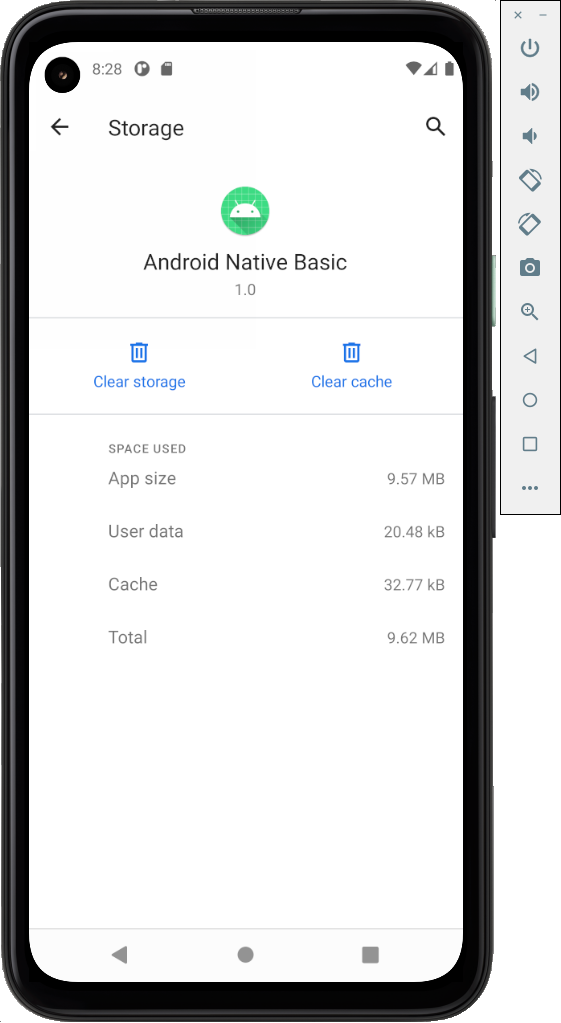
\includegraphics[width=5cm]{img/voefafdruk-a-native-all} }}
    \qquad
    \subfloat[\centering Voetafdruk van de native Android zonder cache en met lokale opslag]{{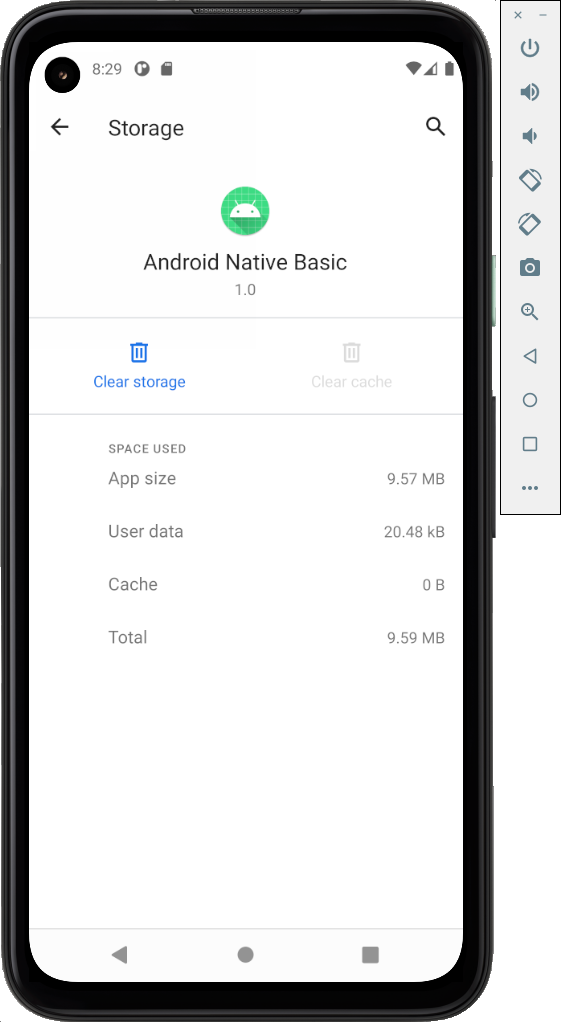
\includegraphics[width=5cm]{img/voefafdruk-a-native-no-cache} }}
    
    \subfloat[\centering Voetafdruk van de native Android zonder cache en lokale opslag]{{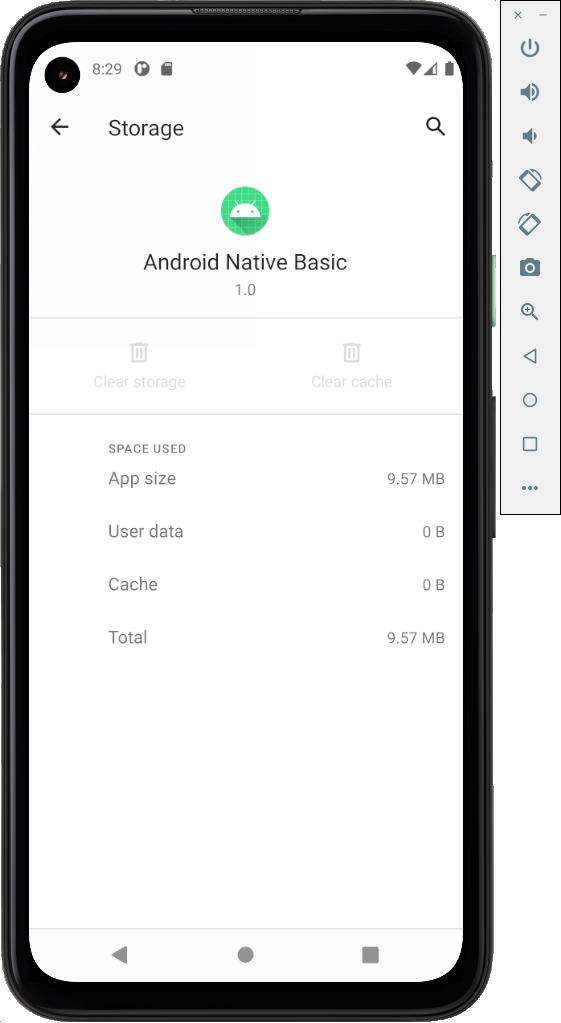
\includegraphics[width=5cm]{img/voefafdruk-a-native-clean} }}
    
    \caption{Voetafdruk van de native Android applicatie}
    \label{fig:M-voetafdruk-android}
\end{figure}


\subsubsection{\IfLanguageName{dutch}{iOS}{iOS}}
\label{sec:M-test-voetafdruk-ios}
De voetafdruk van een iOS applicatie meten is echter niet mogelijk via de emulators binnen Xcode. Om onderstaande resultaten te verzamelen werd gewerkt met een fysiek toestel namelijk de iPhone 11 Pro Max\footnote{support.apple.com/kb/SP806}. De applicatie werd via Xcode op het toestel geïnstalleerd. Daarna kan via de instellingen van de iPhone de grootte van de applicatie bekeken worden.

\begin{figure}
    \centering
    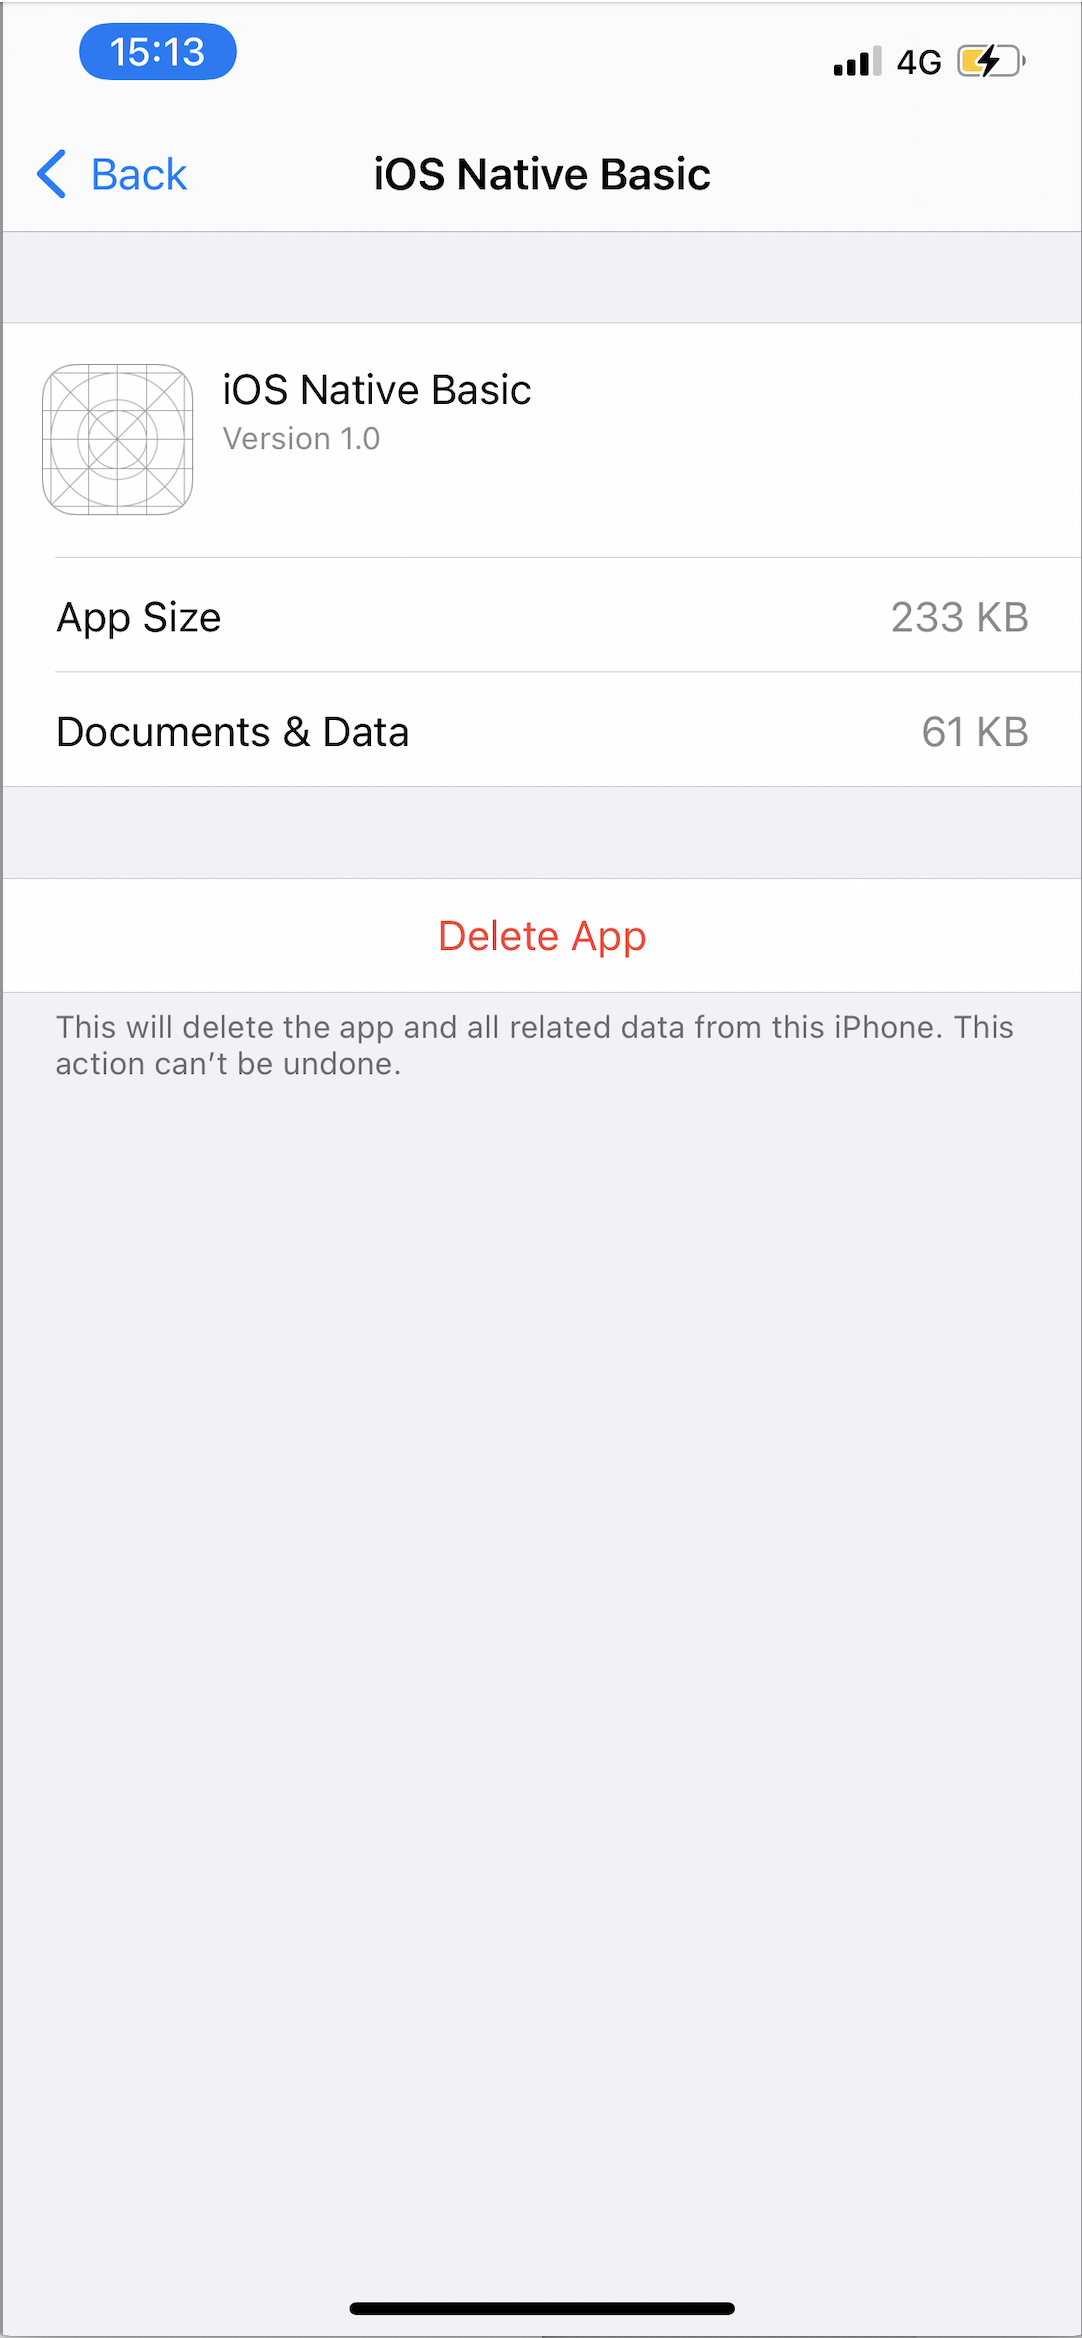
\includegraphics[width=4cm]{img/voetafdruk-i-native}
    \caption{Voetafdruk van de native iOS applicatie}
    \label{fig:M-voetafdruk-ios}
\end{figure}


\subsubsection{\IfLanguageName{dutch}{KMM}{KMM}}
\label{sec:M-test-voetafdruk-kmm}
Zoals reeds vermeld, zal de iOS applicatie geïnstalleerd worden op de fysieke iPhone 11 Pro Max en de Android applicatie op de emulator van binnen Android Studio.

\begin{figure}
    \centering
    \subfloat[\centering Voetafdruk van KMM Android met cache en lokale opslag]{{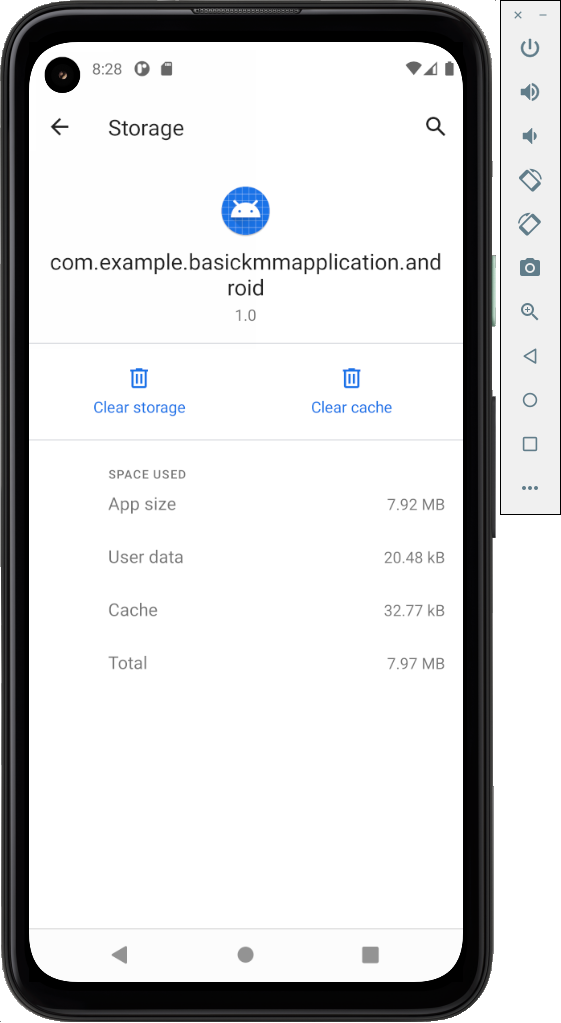
\includegraphics[width=5cm]{img/voefafdruk-kmm-all} }}
    \qquad
    \subfloat[\centering Voetafdruk van KMM Android zonder cache en met lokale opslag]{{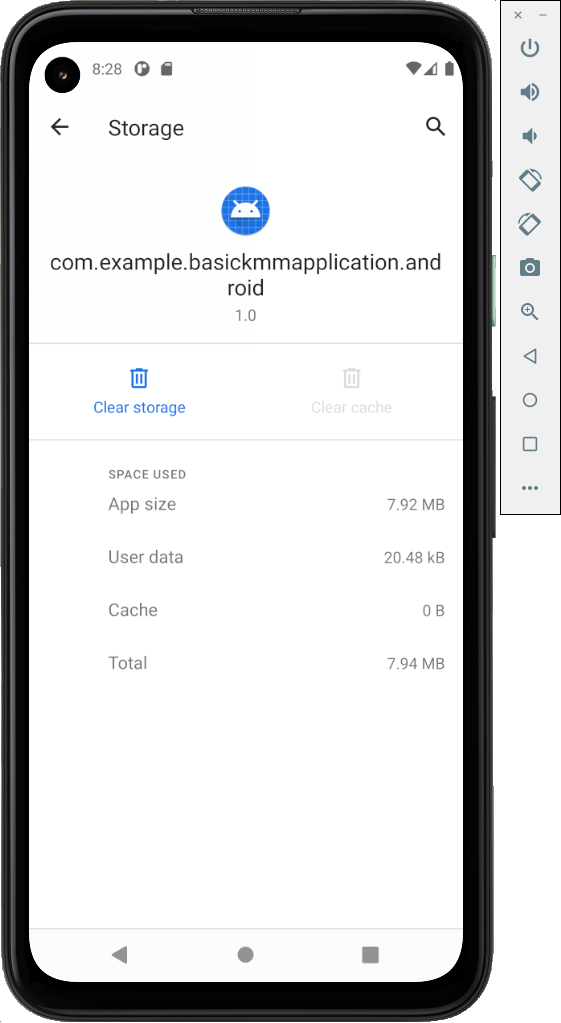
\includegraphics[width=5cm]{img/voefafdruk-kmm-no-cache} }}
    
    \subfloat[\centering Voetafdruk van KMM Android zonder cache en lokale opslag]{{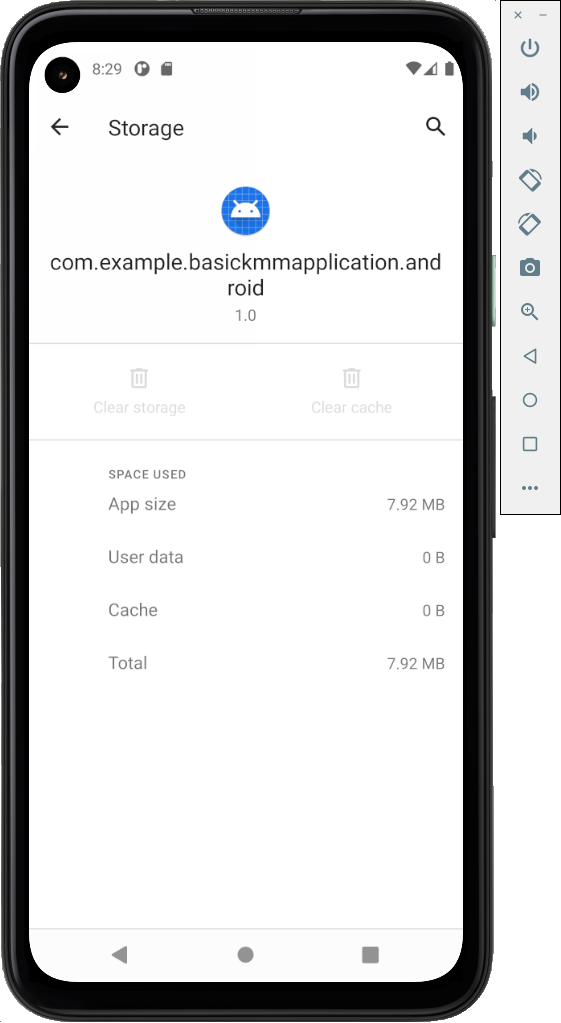
\includegraphics[width=5cm]{img/voefafdruk-kmm-clean} }}
    \qquad
    \subfloat[\centering Voetafdruk van KMM iOS kmm]{{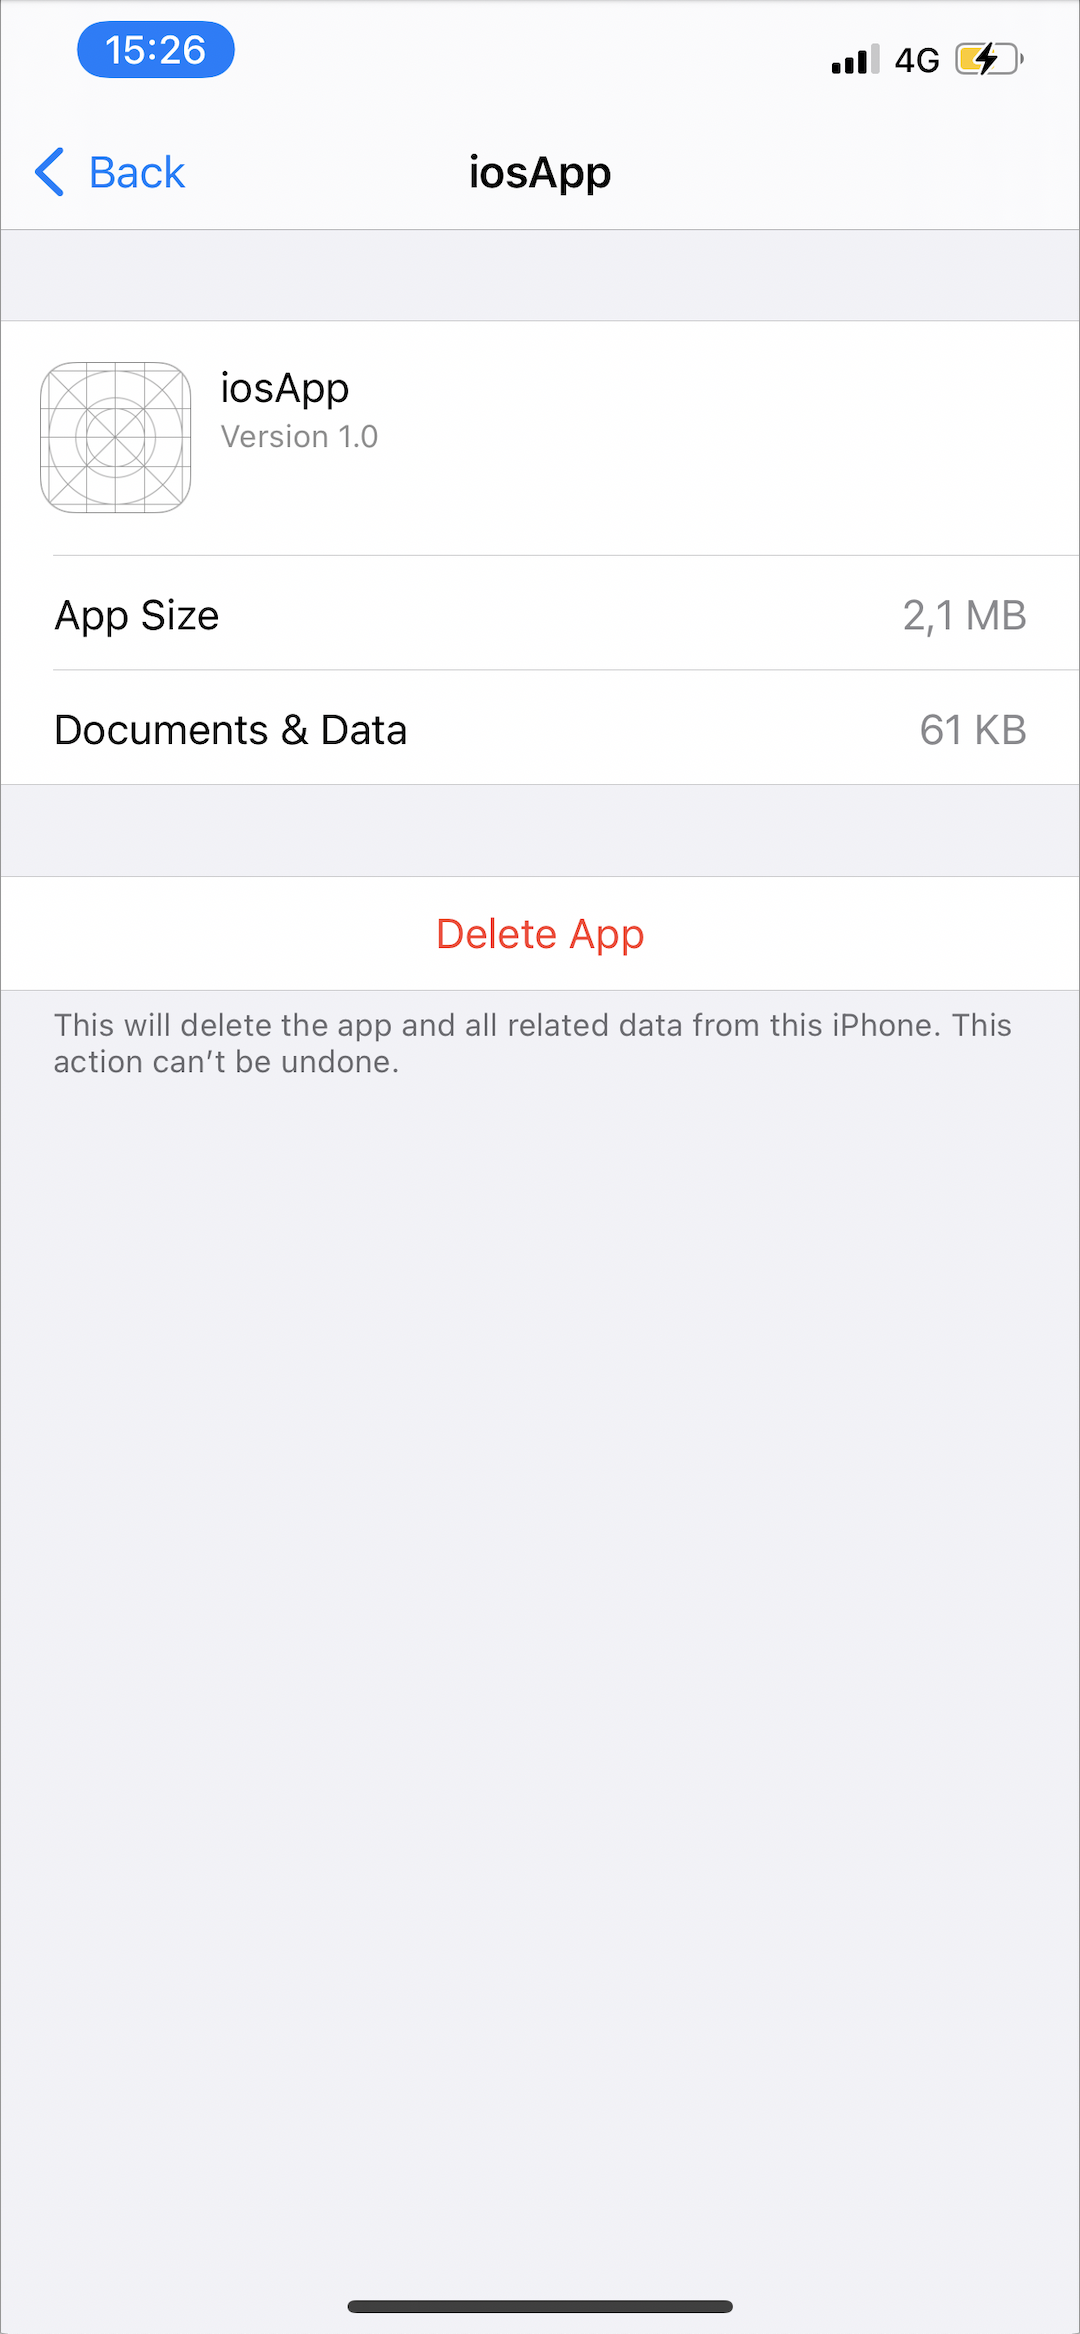
\includegraphics[width=4cm]{img/voetafdruk-i-kmm.png} }}    
    \caption{Voetafdruk van de KMM applicaties}
    \label{fig:M-voetafdruk-kmm}
\end{figure}

\subsubsection{\IfLanguageName{dutch}{Conclusie}{Conclusion}}
\label{sec:M-test-voetafdruk-conclusie}
Bij evaluatie van de resultaten op vlak van voetafdruk, wordt gezien dat KMM Android iets beter scoort dan native, maar dat KMM iOS veel slechter scoort dan native iOS. Tabel \ref{T:voetafruk-overzicht} geeft een overzicht van de voetafdrukken. Om een ander beeld te krijgen, kunnen de waarden van native en KMM opgeteld worden. Hieruit kan dan wel geconcludeerd worden dat native net iets meer performant is op het vlak van de voetafdrukken op de toestellen.


\begin{table}[H]
    \centering
    \caption{Overzicht van de voetafdruk van de applicaties}
    \begin{tabular}{|c|c|c|}
        \hline
        {\textbf{Platform}} & {\textbf{Native}}  & {\textbf{KMM}}\\ \hline \hline
        Android&9,57 MB&7,92 MB\\ \hline
        iOS&0,233 MB&2,1 MB\\ \hline \hline
        \textbf{Totaal}&\textbf{9,803 MB}&\textbf{10,020 MB}\\ \hline
    \end{tabular}
    \label{T:voetafruk-overzicht}
\end{table}

Deze resultaten en conclusie geven een indicatie over wat de verhouding is tussen native en KMM op vlak van de voetafdruk. De waarden zijn echter irrelevant gezien deze aan de hand van meerdere applicaties en over een langere periode dient getest te worden vooraleer hieruit een conclusie kan getrokken worden.

\subsection{\IfLanguageName{dutch}{Ontwikkeltijd}{Development time}}
\label{sec:M-test-ontwikkeltijd}
De ontwikkeltijd is een eerder subjectief gegeven, gezien dit zeer afhankelijk is van de persoon die deze test afneemt. Voor deze studie had de ontwikkelaar geen ervaring met KMM maar wel met Kotlin en Swift. Door de ontwikkelaar waren in het verleden reeds applicaties geschreven voor Android en iOS. De ontwikkeltijden zijn een schatting en omvatten het hele traject van opstart tot het builden van de laatste correcte versie. Deze waarden zijn gebaseerd op commit history en local history binnen de IDE's alsook timetracking van de ontwikkelaar zelf.

\begin{table}[H]
    \centering
    \caption{Overzicht van de ontwikkeltijd van de applicaties}
    \begin{tabular}{|c|c|}
        \hline
        {\textbf{Platform}} & {\textbf{Ontwikkeltijd}}\\ \hline \hline
        Android native&01u 32min\\ \hline
        iOS native&01u 56min\\ \hline
        KMM&3u 26min\\ \hline
    \end{tabular}
    \label{T:ontwikkeltijd-overzicht}
\end{table}

Aan de hand van de resultaten kan geconcludeerd worden dat het voor de ontwikkelaar in de studie net sneller was om een KMM applicatie te maken dan twee native varianten. Een van de belangrijkste zaken hierbij is het feit dat voor native twee projecten moeten opgestart worden. Daarnaast bevatte de KMM applicatie al wat logica op voorhand die kon hergebruikt worden.
\\ \\ 
Indien deze studie zou uitgevoerd worden door een meer ervaren ontwikkelaar die ervaring heeft met Kotlin, Swift en KMM kan verwacht worden dat de KMM applicatie nog sneller ontwikkeld kan worden. De gedeelde domeinlogica kan een heel stuk tijd besparen dit gegeven kwam in dit project ook naar boven kwam.

\subsection{\IfLanguageName{dutch}{Kostprijs}{Cost}}
\label{sec:M-test-lijnen-kostprijs}
Voor de kostprijs zal gebaseerd worden op gegevens die aangereikt werden door Endare, het ondersteunende bedrijf voor deze bachelorproef. Tabel \ref{T:prijzen-overzicht} toont een overzicht van de geschatte kosten. De ontwikkelingstijd wordt gebruikt als basis voor de andere zaken als design, analyse... in te schatten. Deze inschatting gebeurd aan de hand van de ontwikkelingstijd te vermenigvuldigen met een factor van 1,7. Voor de prijs te berekenen werkt Endare met een uurtarief van \euro{} 85 excl. btw.

\begin{table}[H]
    \centering
    \caption{Overzicht van de ontwikkeltijd van de applicaties}
    \begin{tabular}{|c|c|c|c|}
        \hline
        {\textbf{Platform}} & {\textbf{Ontwikkeltijd}}& {\textbf{Totale tijd}}& {\textbf{Prijs (excl. btw)}}\\ \hline \hline
        Android native&01u 32min&2u 36min&\euro{} 221,57\\ \hline
        iOS native&01u 56min&2u 17min&\euro{} 279,37\\ \hline
        KMM&3u 26min&5u 50min&\euro{} 496,12\\ \hline
    \end{tabular}
    \label{T:prijzen-overzicht}
\end{table}

De totale kostprijs voor de twee native applicaties komt dus op \euro{} 500,93 en de KMM applicatie komt op \euro{} 496,12. Het kleine verschil tussen de resultaten is te verklaren door het feit dat gebruik gemaakt is van de resultaten van deel \ref{sec:M-test-ontwikkeltijd}: `Ontwikkeltijd'. Daar werd op het einde ook gewezen op het feit dat bij meer ervaren developers een KMM applicatie interessanter zou zijn. Dit gegeven heeft ook rechtstreeks effect op de prijs, gezien een snellere ontwikkeltijd zorgt voor een lagere prijs.

Uiteindelijk zou ook met het kleine verschil nu de KMM variant goedkoper uitkomen gezien de factor 1,7 geen projectmanagement kosten bevat. Deze kosten zouden in het native verhaal dus twee keer dienen aangerekend te worden en bij de KMM variant maar één keer. Dit maakt dus dat de KMM applicaties goedkoper zal zijn dan de native applicaties.





